\documentclass[12pt]{report}

\newcommand{\fssmall}[0]{\fontsize{8pt}{8pt}\selectfont}
\newcommand{\fsmedium}[0]{\fontsize{10pt}{10pt}\selectfont}

\bibliographystyle{meinbst}
%\bibliographystyle{rmp}
%\bibliographystyle{rusnat}
\usepackage{natbib}
\setcitestyle{aysep={},yysep={, },round,semicolon,authoryear}

\renewcommand{\floatpagefraction}{0.8}
% Mindestgröße Abbildung auf einer eigenen Seite
\renewcommand{\topfraction}{0.85}
\renewcommand{\bottomfraction}{0.5}

\usepackage{float}

\usepackage{amsmath}
\usepackage{hyperref}

%\usepackage[nonumberlist]{glossaries}
%\usepackage{acronym}
%\newglossary[alg]{acronym}{acr}{acn}{\acronymname}
%\newglossary[slg]{symbols}{sls}{slo}{\glssymbolsgroupname}
%\makeglossaries


\usepackage{xfrac}
%\usepackage{nicefrac}

\usepackage{amsmath}
\usepackage{commath}
\usepackage{mathpazo}
%\usepackage{aurical}

\usepackage[utf8]{inputenc}
\usepackage{wrapfig}
\usepackage{subfig}
\usepackage{graphicx}
\graphicspath{{Figures/}}
\usepackage{geometry}
\usepackage{color}

\usepackage{caption}
\captionsetup{font=footnotesize}


        
%\title{
%	{Characterization of nanoparticles by continuous contrast variation in SAXS}\\
%	{\large Physikalisch-Technische Bundesanstalt}\\
%}
%\author{Raul Garcia Diez}
%\date{\today}

\begin{document}
%        %%%%% Glossary entries
\newcommand{\newsymentry}[4]{\newglossaryentry{#1}{name=\ensuremath{#2}, description={#3}, sort=#4, type=symbols}}

%% Acronyms
\newacronym{afm}{AFM}{atomic force microscopy}
\newacronym{asaxs}{ASAXS}{anomalous small-angle X-ray scattering}
\newacronym{bcp}{BCP}{block copolymer}
\newacronym{bessy}{BESSY~II}{electron storage ring for synchrotron radiation}
\newacronym{cd}{CD}{critical dimension}
%\newacronym{com}{COM}{centre of mass}
\newacronym{dft}{DFT}{discrete Fourier transform}
\newacronym{duv}{DUV}{deep ultraviolet}
\newacronym{dwba}{DWBA}{distorted wave Born approximation}
\newacronym{emrp}{EMRP}{European Metrology Research Programme}
\newacronym{euv}{EUV}{extreme ultraviolet}
\newacronym{fcm}{FCM}{four-crystal monochromator}
\newacronym[longplural={free electron lasers},plural={FELs}]{fel}{FEL}{free electron laser}
\newacronym{fem}{FEM}{finite element method}
\newacronym{fft}{FFT}{fast Fourier transformation}
\newacronym{ft}{FT}{Fourier transform}
\newacronym{gisans}{GISANS}{grazing incidence small-angle neutron scattering}
\newacronym{gisaxs}{GISAXS}{grazing incidence small-angle X-ray scattering}
\newacronym[longplural={grating truncation rods},plural={GTRs}]{gtr}{GTR}{grating truncation rod}
\newacronym[sort=GUM]{gum}{GUM}{\textit{Guide to the Expression of Uncertainty in Measurement}}
\newacronym{hzb}{HZB}{Helmholtz-Zentrum Berlin}
\newacronym{itrs}{ITRS}{International Technology Roadmap for Semiconductors}
\newacronym{nist}{NIST}{National Institute for Standards and Technology}
\newacronym[plural={NMIs},longplural={national metrology institutes}]{nmi}{NMI}{national metrology institute}
\newacronym{npl}{NPL}{National Physical Laboratory}
\newacronym[plural={PSDs},longplural={power spectral densities}]{psd}{PSD}{power spectral density}
\newacronym{psf}{PSF}{point spread function}
\newacronym{ptb}{PTB}{Physikalisch-Technische Bundesanstalt}
\newacronym[sort=psbp2vp]{pvp}{\pvp}{polystyrene-\textit{block}-poly(2-vinylpyridine)}
\newacronym{rds}{RDS}{resonant diffuse scattering}
\newacronym{saxs}{SAXS}{small-angle X-ray scattering}
\newacronym{sdd}{SDD}{silicon drift detector}
\newacronym{sem}{SEM}{scanning electron microscopy}
\newacronym{si}{SI system}{International System of Units}
\newacronym{tem}{TEM}{transmission electron microscopy}
\newacronym{uhv}{UHV}{ultra high vacuum}
\newacronym{xanes}{XANES}{X-ray absorption near-edge spectroscopy}
\newacronym{xrr}{XRR}{X-ray reflectometry}


%%% Symbols
\newsymentry{DFT}{\dft{k}}{discrete Fourier transform}{DFT}
\newsymentry{FT}{\ft{\xi}}{Fourier transform of $f(x)$}{FT}
\newsymentry{G}{\ensuremath{G}}{grating groove width}{G}
\newsymentry{H}{\ensuremath{H}}{grating line height}{H}
\newsymentry{P}{\ensuremath{P}}{grating period length (pitch)}{P}
\newsymentry{PSD}{\psd{\xi}}{power spectral density}{PSD}
\newsymentry{CD}{\CD}{critical dimension (grating line width)}{CD}
\newsymentry{Rf}{\vidx{R}{F}}{Fresnel reflectance}{RFresnel}
\newsymentry{R}{\ensuremath{R}}{(specular) reflectance}{R}
\newsymentry{alc}{\alc}{critical angle of total external refraction}{alphac}
\newsymentry{alf}{\alf}{vertical grazing scattering angle with respect to incident beam}{alphaf}
\newsymentry{ali}{\ali}{vertical grazing incidence angle of the X-ray beam}{alphai}
\newsymentry{beta}{\ensuremath{\beta}}{imaginary part of the refractive index, \mbox{$\beta = \Im(\gls{n})$}}{beta}
\newsymentry{c}{\ensuremath{c}}{vacuum speed of light, \mbox{$c = \SI{299792458}{\m\per\s}$}}{c}
\newsymentry{dcs}{\ensuremath{\frac{d\sigma}{d\Omega}}}{differential scattering cross section}{sigmaOmega}
\newsymentry{delta}{\ensuremath{\delta}}{component of the real part of the refractive index, \mbox{$\delta = \Re(\gls{n}) - 1$}}{delta}
\newsymentry{dens}{\dens}{mass density in \si{\kg\per\m\cubed}}{rho}
\newsymentry{edens}{\edens}{electron density, i.e. electrons per unit volume, in \si{\per\m\cubed}}{rhoelectron}
\newsymentry{ematch}{\vidx{E}{match}}{photon energy scattering contrast matching of two materials}{Ematch}
\newsymentry{eph}{\eph}{photon energy of the monochromatic X-ray beam}{Ephoton}
\newsymentry{epsn}{\vidx{\epsilon}{0}}{electric constant (dielectric permittivity of the vacuum), \mbox{$\epsilon_0 = \sfrac{1}{\gls{mun}\gls{c}^2} = \num{8.8541878}\ldots\times10^{-12}\ \si{\farad\per\m}$}}{eps0}
\newsymentry{ethr}{\ethr}{energy threshold setting of the \pil detector, typically $\ethr = \sfrac{1}{2}\, \gls{eph}$}{Ethreshold}
\newsymentry{e}{\ensuremath{e}}{elementary charge, \mbox{$e = \SI{1.602176565(35)e-19}{\ampere\s}$}}{e}
\newsymentry{fwhm}{\vidx{w}{fwhm}}{Bragg peak width}{wfwhm}
\newsymentry{fofac}{\ensuremath{W(\vec{q})}}{effective average particle form factor}{Wfo}
\newsymentry{stfac}{\ensuremath{S(\vec{q})}}{structure factor (interference function)}{Str}
\newsymentry{h}{\ensuremath{h}}{Planck constant, \mbox{$h = \SI{6.62606957(29)e-34}{\joule\s}$}}{h}
\newsymentry{hT}{\vidx{h}{T}}{Tikhonov regularisation parameter}{hT}
\newsymentry{k}{\ensuremath{\vec{k}}}{wave vector; the wave number is \mbox{$|\vec{k}| = k = \sfrac{2\pi}{\gls{lambda}}$}}{k}
\newsymentry{kwidth}{\ensuremath{\gamma}}{width of the Kaiser window}{gamma}
\newsymentry{lambda}{\ensuremath{\lambda}}{wavelength}{lambda}
\newsymentry{lpx}{\lpx}{detector pixel pitch}{Lpx}
\newsymentry{ls}{\ls}{sample-detector distance}{Ls}
\newsymentry{me}{\vidx{m}{e}}{electron rest mass, \mbox{$\vidx{m}{e} = \SI{9.10983291(40)e-31}{\m\per\s}$}}{me}
\newsymentry{mun}{\vidx{\mu}{0}}{magnetic constant (magnetic permeability of the vacuum), \mbox{$\mu_0 = 4 \pi \times 10^{-7}\ \si{\newton\per\ampere\squared}$}}{mu0}
\newsymentry{n}{\n}{complex refractive index, \mbox{$\n = (1-\delta) + i\, \beta$}}{n}
\newsymentry{na}{\vidx{N}{A}}{Avogadro constant, \mbox{$\vidx{N}{A} = \SI{6.02214129(27)e23}{\per\mol}$}}{NA}
\newsymentry{omega}{\ensuremath{\omega}}{wave frequency}{omega}
\newsymentry{pdepth}{\pdepth}{scattering depth}{Lambda}
\newsymentry{phase}{\ensuremath{\vidx{\phi}{phase}}}{phase of electromagnetic wave}{phiphase}
\newsymentry{qc}{\q{c}}{$q$ coordinate at \alf=\alc and/or \ali=\alc}{qc}
\newsymentry{qe}{\qe}{detector quantum efficiency, $\qe = \frac{\text{incoming photons}}{\text{registered photons}}$}{qe}
\newsymentry{qr}{\q{r}}{$q$ at specular condition, $\q{r} = \left.\q{z}\right|_{\alf=\ali}$}{qr}
\newsymentry{q}{\ensuremath{\vec{q}}}{\mbox{scattering vector / reciprocal space vector}, ${\vec{q} = \left(\q{x},\q{y},\q{z}\right)^{T}}$}{q}
\newsymentry{rms}{\vidx{\sigma}{rms}}{root-mean-square interface roughness}{srms}
\newsymentry{rth}{\ensuremath{r_0}}{\mbox{classical electron radius}, \mbox{$r_0 = \SI{2.8179403267(27)e-15}{\m}$}}{rzero}
\newsymentry{thf}{\thf}{azimuthal scattering angle with respect to incident beam}{thetaf}


%% Glossary
\newglossaryentry{pilatus}{name=PILATUS, description={modular two-dimensional hybrid pixel X-ray detector}}
%\newglossaryentry{ewaldsphere}{name=Ewald sphere, description={construct to visualise the occurrence of scattering spots, the radius is $\sfrac{2\pi}\lambda$}}

        %\includeonly{abstract}
        
%        \frontmatter
%            \pagestyle{thesisINTRO}
            % titlepage.tex

\begin{titlepage}
{\noindent\sffamily\large%
    \begin{center}
        \vspace*{3ex}
        {\LARGE\bfseries\sffamily
            Characterization of nanoparticles by continuous contrast variation in small-angle X-ray scattering
        }
        \vspace{1cm}

        vorgelegt von \\
        MSc \\
        Raul Garcia Diez \\
        geboren in Barcelona, Spanien \\
        \vspace{4cm}

        Von der Fakultät II - Mathematik und Naturwissenschaften \\
        der Technischen Universität Berlin \\
        zur Erlangung des akademischen Grades \\
        Doktor der Naturwissenschaften \\
        Dr. rer. nat. \\
        \vspace{3ex}

        genehmigte Dissertation \\
        \vspace{2cm}
    \end{center}

    Promotionsausschuss:
    \vspace{2ex}

    Vorsitzender: Prof. Dr. XXX

    Gutachter: Prof. Dr. Stefan Eisebitt

    Gutachterin: Prof. Dr. Simone Raoux

    Gutachter: Prof. Dr. Mathias Richter
    \vspace{1ex}

    Tag der wissenschaftlichen Aussprache:

    \vfill
    \begin{center}
        Berlin 2016
    \end{center}
}
\end{titlepage}

\cleardoublepage


            \chapter*{Abstract}
\thispagestyle{empty}


In the continuously growing field of nanomedicine, nanonoparticles have a preeminent position, opening exciting new possibilities as platforms for drug-delivery or encapsulating imaging agents. Indeed, polymeric colloids are starting to undergo clinical trials and a lipid vesicle was used as nanocarrier for the first approved nano-drug, Doxil. Therefore, the current advances in nanomaterial development are focused towards tailoring polymeric nano-drug carriers with flexible surface functionalization and controlled morphologies, defining aspects of the particle functions e.g. their \emph{in vivo} biodistribution or their drug-delivery efficacy. 

However, most current characterization techniques possess certain limitations i.e. cannot prove the innner structure present in many low-density nanoparticles. This work proposes a novel approach to contrast variation with SAXS \textbf{[1]} based on the constitution of a solvent density gradient in a glass capillary in order to choose \emph{in situ} the most appropriate contrast and to acquire extensive datasets in a short time interval.

By examining the scattering curves measured at different aqueous sucrose densities, information about the internal morphology of the nanoparticles as well as their size distribution can be obtained. Additionally an estimation of the particle density can be determined focusing on the Guinier region of the curve, as shown for polymeric colloids across a wide spectrum of polymers \textbf{[2]}. These results were successfully compared with techniques such as DCS and several imaging methods.

The continuous contrast variation technique was also employed to characterize the nano-drug Doxil$\textregistered$, a PEGylated liposomal formulation of doxorubicin, using iodixanol as contrast agent, an iso-osmolar suspending medium. The study is focused on the isoscattering point position and the model-free analysis of the scattering curves and highlights the advantages in comparison to widespread characterization techniques as DLS and TEM \textbf{[3]}.

Furthermore, the response of the nanocarrier to increasing solvent osmolality is evaluated with sucrose contrast variation and compared to the different response of PEGylated and plain liposomes to osmotic pressure depending on their size. The osmotic pressure needed for the liposomal shrinkage is quantitatively studied by focusing on the evolution of the isoscattering point intensity, while the study of the phospholipid bilayer scattering feature gives an insight into the morphological changes induced by the osmotic shrinkage.

The possibilities as sizing technique of the continuous contrast variation method are further investigated on relevant bio-materials like human lipoproteins or polymeric nanocarriers coated with antibodies. In addition, this technique is employed to determine the density of the lipoproteins, one of the most characteristic traits of these blood plasma components.

\bigskip
\footnotesize{

\textbf{[1]} R. Garcia-Diez, C. Gollwitzer, M. Krumrey, \emph{J. Appl. Cryst.} \textbf{48}, 20-28 (2015)

\textbf{[2]} R. Garcia-Diez, A. Sikora, C. Gollwitzer, C. Minelli, M. Krumrey, \emph{Eur. Polym. J.} \textbf{81}, 641-649 (2016)

\textbf{[3]} R. Garcia-Diez, C. Gollwitzer, M. Krumrey, Z. Varga, \emph{Langmuir} \textbf{32 (3)}, 772-778 (2015)

}
\normalsize

\cleardoublepage

\thispagestyle{empty}
\selectlanguage{ngerman}

\chapter*{Zusammenfassung}

\textcolor{red}{A GOOD TRANSLATION WILL BE DONE ONCE THE ENGLISH ABSTRACT IS DEFINITIVE! THAT WAS ONLY GOOGLE TRANSLATOR!!!}Im kontinuierlich wachsenden Bereich der Nanomedizin haben Nanopartikel eine herausragende Stellung und eröffnen aufregende neue Möglichkeiten als Plattform für Wirkstoffabgabe oder Verkapselung bildgebender Mittel. Tatsächlich beginnen polymere Kolloide, klinische Versuche durchzuführen, und ein Lipidvesikel wurde als Nanoträger für das erste zugelassene Nano-Medikament (Doxil) verwendet. Daher sind die gegenwärtigen Fortschritte in der Entwicklung von Nanomaterialien darauf ausgerichtet, polymere Nano-Arzneimittelträger mit flexibler Oberflächenfunktionalisierung und gesteuerten Morphologien herzustellen, wobei Aspekte der Teilchenfunktionen, z.B. Ihre \emph{in vivo}-Bioverteilung oder ihre Wirksamkeit bei der Wirkstoffabgabe.

Jedoch besitzen die meisten gegenwärtigen Charakterisierungstechniken gewisse Beschränkungen, d.h. nicht die innere Struktur beweisen, die in vielen Nanopartikeln niedriger Dichte vorhanden ist. Diese Arbeit schlägt einen neuen Ansatz zur Kontrastveränderung mit SAXS auf der Grundlage des Aufbaus eines Lösungsmitteldichtegradienten in einer Glaskapillare vor \textbf{[1]}, um \emph{in situ} den geeignetsten Kontrast zu wählen und umfangreiche Datensätze in einem kurzen Zeitintervall zu erwerben.

Durch Untersuchung der bei unterschiedlichen wässrigen Sucrose-Dichten gemessenen Streukurven können Informationen über die innere Morphologie der Nanopartikel sowie deren Größenverteilung erhalten werden. Zusätzlich kann eine Schätzung der Partikeldichte mit Fokussierung auf den Guinier-Bereich der Kurve, wie für polymere Kolloide über ein breites Spektrum von Polymeren gezeigt, bestimmt werden \textbf{[2]}. Diese Ergebnisse wurden erfolgreich mit Techniken wie DCS und mehrere bildgebende Verfahren verglichen.

Die kontinuierliche Kontrastveränderungstechnik wurde ebenfalls verwendet, um Doxil, eine PEGylierte liposomale Formulierung von Doxorubicin, unter Verwendung von Iodixanol als Kontrastmittel, eines iso-osmolaren Suspensionsmediums, zu charakterisieren. Die Studie konzentriert sich auf die Isoscattering-Point-Position und die modellfreie Analyse der Streukurven und hebt die Vorteile im Vergleich zu weit verbreiteten Charakterisierungstechniken als DLS und TEM hervor \textbf{[3]}.

Darüber hinaus wird die Reaktion des Nanoträgers auf die zunehmende Lösungsmittel-Osmolalität mit einer Saccharose-Kontrast-Variation bewertet und mit der unterschiedlichen Reaktion von PEGylierten und einfachen Liposomen auf den osmotischen Druck in Abhängigkeit von ihrer Größe verglichen. Der für die liposomale Schrumpfung benötigte osmotische Druck wird quantitativ durch die Fokussierung auf die Evolution der Isoscattering-Punkt-Intensität untersucht, während die Untersuchung der Phospholipid-Doppelschicht-Streuung einen Einblick in die morphologischen Veränderungen der osmotischen Schrumpfung gibt.

Die Möglichkeiten der Dimensionierung des kontinuierlichen Kontrastvariationsverfahrens werden auch auf relevanten Biomaterialien wie menschlichen Lipoproteinen oder mit Antikörpern beschichteten polymeren Nanocarrieren gezeigt. Zusätzlich wird diese Technik verwendet, um die Dichte der Lipoproteine zu bestimmen, eine der charakteristischsten Merkmale dieser Blutplasmakomponenten.

\bigskip
\footnotesize{

\textbf{[1]} R. Garcia-Diez, C. Gollwitzer, M. Krumrey, \emph{J. Appl. Cryst.} \textbf{48}, 20-28 (2015)

\textbf{[2]} R. Garcia-Diez, A. Sikora, C. Gollwitzer, C. Minelli, M. Krumrey, \emph{Eur. Polym. J.} \textbf{81}, 641-649 (2016)

\textbf{[3]} R. Garcia-Diez, C. Gollwitzer, M. Krumrey, Z. Varga, \emph{Langmuir} \textbf{32 (3)}, 772-778 (2015)

}
\normalsize

\selectlanguage{UKenglish}
\cleardoublepage
        
%	\maketitle
%	\chapter*{Abstract}
\thispagestyle{empty}


In the continuously growing field of nanomedicine, nanonoparticles have a preeminent position, opening exciting new possibilities as platforms for drug-delivery or encapsulating imaging agents. Indeed, polymeric colloids are starting to undergo clinical trials and a lipid vesicle was used as nanocarrier for the first approved nano-drug, Doxil. Therefore, the current advances in nanomaterial development are focused towards tailoring polymeric nano-drug carriers with flexible surface functionalization and controlled morphologies, defining aspects of the particle functions e.g. their \emph{in vivo} biodistribution or their drug-delivery efficacy. 

However, most current characterization techniques possess certain limitations i.e. cannot prove the innner structure present in many low-density nanoparticles. This work proposes a novel approach to contrast variation with SAXS \textbf{[1]} based on the constitution of a solvent density gradient in a glass capillary in order to choose \emph{in situ} the most appropriate contrast and to acquire extensive datasets in a short time interval.

By examining the scattering curves measured at different aqueous sucrose densities, information about the internal morphology of the nanoparticles as well as their size distribution can be obtained. Additionally an estimation of the particle density can be determined focusing on the Guinier region of the curve, as shown for polymeric colloids across a wide spectrum of polymers \textbf{[2]}. These results were successfully compared with techniques such as DCS and several imaging methods.

The continuous contrast variation technique was also employed to characterize the nano-drug Doxil$\textregistered$, a PEGylated liposomal formulation of doxorubicin, using iodixanol as contrast agent, an iso-osmolar suspending medium. The study is focused on the isoscattering point position and the model-free analysis of the scattering curves and highlights the advantages in comparison to widespread characterization techniques as DLS and TEM \textbf{[3]}.

Furthermore, the response of the nanocarrier to increasing solvent osmolality is evaluated with sucrose contrast variation and compared to the different response of PEGylated and plain liposomes to osmotic pressure depending on their size. The osmotic pressure needed for the liposomal shrinkage is quantitatively studied by focusing on the evolution of the isoscattering point intensity, while the study of the phospholipid bilayer scattering feature gives an insight into the morphological changes induced by the osmotic shrinkage.

The possibilities as sizing technique of the continuous contrast variation method are further investigated on relevant bio-materials like human lipoproteins or polymeric nanocarriers coated with antibodies. In addition, this technique is employed to determine the density of the lipoproteins, one of the most characteristic traits of these blood plasma components.

\bigskip
\footnotesize{

\textbf{[1]} R. Garcia-Diez, C. Gollwitzer, M. Krumrey, \emph{J. Appl. Cryst.} \textbf{48}, 20-28 (2015)

\textbf{[2]} R. Garcia-Diez, A. Sikora, C. Gollwitzer, C. Minelli, M. Krumrey, \emph{Eur. Polym. J.} \textbf{81}, 641-649 (2016)

\textbf{[3]} R. Garcia-Diez, C. Gollwitzer, M. Krumrey, Z. Varga, \emph{Langmuir} \textbf{32 (3)}, 772-778 (2015)

}
\normalsize

\cleardoublepage

\thispagestyle{empty}
\selectlanguage{ngerman}

\chapter*{Zusammenfassung}

\textcolor{red}{A GOOD TRANSLATION WILL BE DONE ONCE THE ENGLISH ABSTRACT IS DEFINITIVE! THAT WAS ONLY GOOGLE TRANSLATOR!!!}Im kontinuierlich wachsenden Bereich der Nanomedizin haben Nanopartikel eine herausragende Stellung und eröffnen aufregende neue Möglichkeiten als Plattform für Wirkstoffabgabe oder Verkapselung bildgebender Mittel. Tatsächlich beginnen polymere Kolloide, klinische Versuche durchzuführen, und ein Lipidvesikel wurde als Nanoträger für das erste zugelassene Nano-Medikament (Doxil) verwendet. Daher sind die gegenwärtigen Fortschritte in der Entwicklung von Nanomaterialien darauf ausgerichtet, polymere Nano-Arzneimittelträger mit flexibler Oberflächenfunktionalisierung und gesteuerten Morphologien herzustellen, wobei Aspekte der Teilchenfunktionen, z.B. Ihre \emph{in vivo}-Bioverteilung oder ihre Wirksamkeit bei der Wirkstoffabgabe.

Jedoch besitzen die meisten gegenwärtigen Charakterisierungstechniken gewisse Beschränkungen, d.h. nicht die innere Struktur beweisen, die in vielen Nanopartikeln niedriger Dichte vorhanden ist. Diese Arbeit schlägt einen neuen Ansatz zur Kontrastveränderung mit SAXS auf der Grundlage des Aufbaus eines Lösungsmitteldichtegradienten in einer Glaskapillare vor \textbf{[1]}, um \emph{in situ} den geeignetsten Kontrast zu wählen und umfangreiche Datensätze in einem kurzen Zeitintervall zu erwerben.

Durch Untersuchung der bei unterschiedlichen wässrigen Sucrose-Dichten gemessenen Streukurven können Informationen über die innere Morphologie der Nanopartikel sowie deren Größenverteilung erhalten werden. Zusätzlich kann eine Schätzung der Partikeldichte mit Fokussierung auf den Guinier-Bereich der Kurve, wie für polymere Kolloide über ein breites Spektrum von Polymeren gezeigt, bestimmt werden \textbf{[2]}. Diese Ergebnisse wurden erfolgreich mit Techniken wie DCS und mehrere bildgebende Verfahren verglichen.

Die kontinuierliche Kontrastveränderungstechnik wurde ebenfalls verwendet, um Doxil, eine PEGylierte liposomale Formulierung von Doxorubicin, unter Verwendung von Iodixanol als Kontrastmittel, eines iso-osmolaren Suspensionsmediums, zu charakterisieren. Die Studie konzentriert sich auf die Isoscattering-Point-Position und die modellfreie Analyse der Streukurven und hebt die Vorteile im Vergleich zu weit verbreiteten Charakterisierungstechniken als DLS und TEM hervor \textbf{[3]}.

Darüber hinaus wird die Reaktion des Nanoträgers auf die zunehmende Lösungsmittel-Osmolalität mit einer Saccharose-Kontrast-Variation bewertet und mit der unterschiedlichen Reaktion von PEGylierten und einfachen Liposomen auf den osmotischen Druck in Abhängigkeit von ihrer Größe verglichen. Der für die liposomale Schrumpfung benötigte osmotische Druck wird quantitativ durch die Fokussierung auf die Evolution der Isoscattering-Punkt-Intensität untersucht, während die Untersuchung der Phospholipid-Doppelschicht-Streuung einen Einblick in die morphologischen Veränderungen der osmotischen Schrumpfung gibt.

Die Möglichkeiten der Dimensionierung des kontinuierlichen Kontrastvariationsverfahrens werden auch auf relevanten Biomaterialien wie menschlichen Lipoproteinen oder mit Antikörpern beschichteten polymeren Nanocarrieren gezeigt. Zusätzlich wird diese Technik verwendet, um die Dichte der Lipoproteine zu bestimmen, eine der charakteristischsten Merkmale dieser Blutplasmakomponenten.

\bigskip
\footnotesize{

\textbf{[1]} R. Garcia-Diez, C. Gollwitzer, M. Krumrey, \emph{J. Appl. Cryst.} \textbf{48}, 20-28 (2015)

\textbf{[2]} R. Garcia-Diez, A. Sikora, C. Gollwitzer, C. Minelli, M. Krumrey, \emph{Eur. Polym. J.} \textbf{81}, 641-649 (2016)

\textbf{[3]} R. Garcia-Diez, C. Gollwitzer, M. Krumrey, Z. Varga, \emph{Langmuir} \textbf{32 (3)}, 772-778 (2015)

}
\normalsize

\selectlanguage{UKenglish}
\cleardoublepage

	
	\tableofcontents
%	\printglossary[type=\acronymtype,title=Abbreviations,style=list]
%	\printglossary[type=symbols,title=Symbols,style=long,nonumberlist=true]
	
	\section*{Abbreviations}

\thispagestyle{empty}


SAXS Small-angle X-ray Scattering

DCS Differential Centrifugal Sedimentation

	\section*{Symbols}

\begin{itemize}
        
        \item[$a$] Lattice constant of the crystal
        \item[$A$] Atomic mass
        \item[$B$] Magnetic field strength of the bending magnet
        \item[$c$] Speed of light in vacuum     
        \item[$D$] Characteristic length of an object
        \item[$\sfrac{d\sigma}{d\Omega}$] Differential scattering cross-section   
        \item[$\Delta\eta$] Scattering contrast        
        \item[$e$] Charge of the electron  
        \item[eV] Electronvolt
        \item[$E$] Photon's energy
        \item[$E_c$] Critical energy of the bending magnet
        \item[$\epsilon_0$] Vacuum permittivity
        \item[$\eta$] Dynamic viscosity of a fluid 
        \item[$f$] Scattering amplitude or form factor
        \item[$f_0$] Scattering amplitude at the limit $\vect{q}\rightarrow 0$
        \item[$f',f''$] Real and imaginary part of the anomalous scattering coefficient
        \item[$g$] Size distribution fucntion
        \item[$h$] Planck's constant          
        \item[$\hbar$] Reduced Planck's constant, defined as $\hbar = \sfrac{h}{2 \pi}$
        \item[$I$] Scattering intensity
        \item[$I_s$] Shape scattering function or resonant term
        \item[$k=\abs{\vect{k}}$] Photons's wavenumber
        \item[$K$] Deflection parameter of the insertion device
        \item[$K_B$] Boltzmann constant
        \item[$\lambda$] Photon's wavelength  
        \item[$m_e$] Electron mass
        \item[$\mu$] Attenuation coefficient
        \item[$n$] Refractive index        
        \item[$N$] Number of particles
        \item[$N_A$] Avogadro constant
        \item[$p_d$] Polydispersity degree
        \item[$q$] Momentum transfer 
        \item[$q^{\star}$] Isoscattering point
        \item[$r_e$] Classical electron radius          
        \item[$R$] Radius of the particle 
        \item[$R_g$] Radius of gyration 
        \item[$\overline{R}$] Mean radius of the particle size distribution
        \item[$\rho_0$] Average electron density of the particle
        \item[$\rho_e$] Electron density
        \item[$\rho_{\text{solv}}$] Electron density of the suspending medium
        \item[$\rho$] Mass density
        \item[$\sigma$] Attenuation cross-section
        \item[$\sigma_R$] Standard deviation of the particle size distribution
        \item[$T$] Temperature  
        \item[2$\theta$] Scattering angle
        \item[$V$] Volume
        \item[$\tilde X$] Intensity-weighted average of the parameter $X$
        \item[$Z$] Atomic number

\end{itemize}

\cleardoublepage

		
%	\mainmatter
	
	\chapter{Introduction: Nanoparticles in medicine and biology}
The morphology of nanoparticles determines the properties necessary for their utilization in real-world applications. For instance, in drug delivery devices the phenomena involved in biocompatibility reactions (e.g. protein adsorption) depend on the amount of available surface and the nanoparticles' properties \citet{vittaz_effect_1996}. Particularly, polymer lattices and biodegradable nanoparticles have been of growing importance of late as drug carriers \citet{kattan_phase_1992} and thus extensively characterized \citet{soppimath_biodegradable_2001}. The size determination and the characterization of the radial structure of the particles are therefore fundamental tasks. 
\label{chap:introduction}

\section{Polymeric colloids}
\subsection{Functionalization for protein binding}

\subsection{Polymerization consequences}
initiator, co-monomer, surfactants

\section{Liposomal nanocarriers}
formation from amphiphilic lipids
\subsection{Phospholipid bilayer}
typical lipid HSPC, DPPC, cholesterol, PEG

\subsection{polydispersity control}
extrusion, paper with zoltan about scattering in SSLs

\subsection{Drug carrier and SSLs}
stealth function, bilayer stability, filling with pH gradient

\section{Physicochemical characterization}
\subsection{Dimensional metrology and traceability}

\subsection{Characterization tools}
\subsubsection{Single-particle method}
AFM, TEM, SEM, TSEM

\subsubsection{Ensemble methods}
DLS, DCS, SAXS



	
	\chapter{Theoretical Background}
\label{chap:theory_SAXS}

\section{Interaction of light/X-ray and matter}

X-rays can be considered a wave in vacuum with a wave vector 

\begin{equation}
        k=\abs{\vec{k}} = \frac{2\pi}{\lambda}
\end{equation}

The photon energy can be related to this wave length by using the following formula, which uses the quantisation of light/electromagneti radiation as an ensemble of quanta or photons

\begin{equation}
        \lambda = \frac{h c}{E_{ph}}
\end{equation}

The x-rays are an electromagnetic wave. The primary wave irradiating the sample is assumed plane and monochromatic

\begin{equation}
        \vec{E_i}\left( \vec{r},t \right)=\vec{E_i}e^{-i\left( \omega t - \vec{k_i}\vec{r} \right)}
\end{equation}

\subsection{Beer-Lambert law}
\label{sec:BeerLambert}

the attenuation of light to the properties of the material 

When the X-ray beam passes through the material, it transfers energy to the absorbing matter, attenuating its original intensity depending on the volume of the absorbing element. The decrease in the intensity is directly proportional to the concentration of the absorber C and the path length of the X-ray inside the sample dx.

intensity through the sample

\begin{equation}
        dI\left( x \right)=-\mu I dx
\end{equation}
where $\mu$ is the linear absorption coefficient.
\begin{equation}
        I\left( x \right)=I_0e^{-\mu x}
\end{equation}

For x-rays, the refractive index is very close to 1 because $\delta\simeq10^{-5}$. Refraction can be neglected and we can focus on the scattering experimetns

\begin{equation}
        n = 1 - \delta +i \beta
\end{equation}

The X-ray can interact in 3 different ways with the electron. 3 mechanisms.

- Photoelectron absorption

- Inelastic scattering (compton scattering): in this case, it can be neglected because $E_{ph}<<< m_ec^2$ . We are not treating it, because we are just using X-ray. Compton scattering is almost negligible at low angles , where the scattered photon has a different wavelength than the incident photon $\lambda$

\begin{equation}
        \lambda_{scat}-\lambda = \frac{h}{m_e c}\left( 1 - \cos{\Theta} \right) \simeq \frac{h}{2m_e c} \Theta ^ 2
\end{equation}

- Elastic scattering: Is the intersting part for SAXS

The attenuation of light in matter is a combination of these 3 effects, as seen here: $\mu$ linear attenuation coefficient $\tau_{abs}$ photoelectron absorption cross-section $\sigma_{scat}$ scattering cross-section

\begin{equation}
        \mu = \rho_e (\tau_{abs}+\sigma_{scat, el}+\sigma_{scat, inel})
\end{equation}

If there is more than one element inside

\begin{equation}
        \mu = \sum_i \mu_i
\end{equation}

In the case of electrons, 
\begin{equation}
        \mu_i = \rho_{e} \sigma_a
\end{equation}

where $\rho_{at}$ is the atomic/ELECTRON number density and $\sigma_a$ the corresponding atomic cross-section

The electron density is related to the mass density
\begin{equation}
        \rho_e = \rho N_A \frac{Z}{A}
\end{equation}
\begin{equation}
        \mu = \sum_i \sigma_i \rho_i =\sigma_i \frac{C_i}{N_A}
\end{equation}
where $C_I$ is the concentration of scatteres. Therefore, the Beer-Lambert law for different elements in the solution (for example, water and solute):

\begin{equation}
        I = = I_0 e^{\mu}=e^{\mu_solv}e^{\mu_solute}
\end{equation}

\subsection{Photoelectron absorption}

xray photon is absorbed by an atom and the excess energy is transferred to an electron, whih is expelled from the atom, leaving it ionized.

Photon completely absorbed

Fluorescence, Auger electorn

\subsection{Elastic scattering}

\subsubsection{Thompson scattering}
Elastic scattering by a free electron

Intensity of the secondary/scattered wave by classical theory (for an unpolarized light)

\begin{equation}
        I_{scat}\left( r \right)= I_0 \left( \frac{e^2}{4\pi \epsilon_0 m c^2} \right)^2 \frac{1}{r^2} \left( \frac{1+\cos^2{2\Theta}}{2} \right)
\end{equation}

where the Thomson radius, classical electron radius is $2.82\cdot10^{-15}$ m is defined by:

\begin{equation}
        r_e= \frac{e^2}{4\pi\epsilon_0 m c^2}
\end{equation}

The differential scattering cross section is defined by:

\begin{equation}
        \frac{d\sigma}{d\Omega}= \frac{I_{scat} \cdot \left(r^2 \Delta \Omega \right)}{I_0\Delta \Omega}=r_e^2\left( \frac{1+\cos^2{2\Theta}}{2} \right)
\end{equation}


\textcolor{blue}{THIS DOES NOT BELONG HERE: The minus symbols means that the phase between the incident and the scattered photon is dephased by $\pi$}

\subsubsection{Rayleigh scattering}
Scattered by an ensemble of electrons.

Fraunhoffer approximation where the detection point is at a distance L which is much larger than the scattering object size d $d<<<L$ and therefore $\abs{\vec{r}-\vec{r'}}=r$

\textcolor{red}{GRAPH WITH SCATTERING ANGLE AND CONTINUUM OBJECT WHERE THE POSITIONS ARE DEFINED: R AND R'}

Mie scattering: Differences depend on wavelength and size of the object

\section{Small-angle X-ray scattering}
\subsection{Physical process}
\subsection{Evaluation of the scattering intensity}
Form factor * S(q)
Electron density
Number of colloids
\subsubsection{What is $q$?}
The momentum transfer \(q\) of the scattering curves was calculated using
\begin{equation}
q=\frac{4\pi E}{hc}\sin\theta ,
\end{equation}
where \(\theta\) is half of the scattering angle, \(h\) is the Planck constant and \(c\) is the speed of light.

\subsubsection{Modelling of the scattering curve}
What about size distributions? Log-normal, gaussian, Monte-carlo free number of sizes (Pauw)

The scattering intensity of an ensemble of randomly oriented nanoparticles in suspension can be expressed as a function of the momentum transfer \( q \), modulus of the scattering vector \(\vec q\), as
\begin{equation}
\label{eq:intensity}
I(q)=N\int_{0}^{\infty} g(R)\left|F(q,R) \right|^2 dR,
\end{equation}
where \(N\) is the number of scatterers, \(g(R)\) is the size distribution function and \(F(R)\) is the particle form factor, which depends on the inner radial structure of the particle. If the particle shows a heterogeneous morphology, the form factor differs qualitatively for different suspending medium densities.  For sufficiently monodisperse particle suspensions, the Fourier region of the scattering curve shows pronounced minima that characterize the particle structure. 

For a typical morphology with sharp interfaces between the radial symmetric components of the particle with radius \(R_i\) the form factor is
\begin{equation}
\label{eq:multicore-shell}
F\left(q,R \right)= \Delta \eta f_{sph}(q,R)+\sum_{i=1}^{n-1} \Delta\rho_i \left( f_{sph}(q,R_{i+1})-f_{sph}(q,R_{i}) \right) ,
\end{equation}
where \(R\) is the external radius of the particle, \( n \) is the number of concentric shells and \(f_{sph}\) is the form factor of a homogeneous solid sphere given by
\begin{equation}
f_{sph}(q,R)=\frac{4}{3} \pi R^3  \left( 3\frac{\sin{qR}-qR\sin{qR}}{(qR)^3}\right).
\label{eq:ff_sph}
\end{equation}
\begin{itemize}
	\item [Sphere] Gudrun polymeric colloids???
	
	In the case of the PMMA-COOH colloids, the form factor is calculated for a homogeneous solid sphere with electron density $\rho_0$:
\begin{equation}
f_{sph}(q,R)=\frac{4}{3} \pi R^3  \left( 3\frac{\sin{qR}-qR\cos{qR}}{(qR)^3}\right)=\frac{F(q,R)}{\rho_0}.
\label{eq:ff_sph}
\end{equation}
	\item [Core-shell] Interface effects???
	
	The model represents a radially symmetric particle with a sharp interface between the outer shell and the inner core. The form factor is described by

\begin{equation}
	\begin{split}
	F(q,R)= & \Delta\eta f_{sph}(q,R)+ \\
	& \Delta\rho\left[ f_{sph}(q,R)-f_{sph}(q,R_{core}) \right] ,
	\end{split}
\label{eq:ff_cs}
\end{equation}

where \(R \) and \(R_{core} \)  are the outer shell and inner core radii respectively, the excess of electron density is \(\Delta\rho=\rho_{shell}-\rho_{core}\) and the contrast is expressed as \(\Delta\eta=\rho_{core}-\rho_{solv}\), where $\rho_{solv}$ is the electron density of the suspending medium.

	\item [Onion model] It can be used for single-SAXS experiment maybe
	\item [Vesicle] 5 gaussian????
	\item [Inclusion of background] a+b*q-4
	\item [Double shell model] Used in the protein-coated Kisker NPs (last chapter)
\end{itemize}

\subsubsection{Guinier approximation}
deviation when using too few point
Polydispersity effects

\section{Contrast variation}
Solvent variation

ASAXS

When analyzing contrast variation data, a widespread theoretical approach is based in the non-interacting model proposed by Stuhrmann $\&$ Kirste \citeyear{stuhrmann_elimination_1965,stuhrmann_elimination_1967} for monodisperse particles. The so-called \emph{basic functions} formulation differentiates, independently of the particle inner structure, the contributions which depend on the varying solvent density or contrast (\(\Delta\eta=\rho_{core}-\rho_{solv}\)) and on the excess of electron density of each component \(\Delta \rho_i =\rho_i-\rho_{core}\). 
\subsection{Isoscattering point}
One of the best known features appearing in a contrast variation experiment is the existence of \emph{isoscattering points}. At these specific \( q\)-values, the scattering intensity is independent of the adjusted solvent contrast, i.e. all scattering curves intersect in the isoscattering points regardless of the contrast. The isoscattering points \(q^{\star}\) are particularly interesting because they emerge for any spherical particle with an inner structure and a sufficiently narrow size distribution. From the contrast-depending part of equation \eqref{eq:multicore-shell}, a model-free expression can be derived which relates the position of the isoscattering points \(q^{\star}_i\) with the external radius of the particle \( R \), independent of its radial structure \cite{kawaguchi_isoscattering_1992}:
\begin{equation}
\label{eq:isoscattering}
\tan(q^{\star}_iR)=q^{\star}_iR
\end{equation}
The positions of the isoscattering points correspond to the minima positions of the scattering intensity of a compact spherical particle with radius \( R \). Although this expression is derived for the monodisperse case, it can still be applied up to a moderate degree of polydispersity, if care is taken regarding the shift of the minima position due to polydispersity \cite{beurten_polydispersity_1981}. If defining the polydispersity degree \( p_d\) as the full width half maximum of the particle size distribution divided by its average value, for size distributions with \( p_d\) larger than \( \approx 30\,\% \), the isoscattering point is not well defined and the intersection point of the curves is smeared out, showing a diffuseness in the isoscattering point position \cite{kawaguchi_isoscattering_1992}.
\subsubsection{Possible deviations}
Polydispersity and ellipticity smearing (simulation, calculation)
\subsection{Basic functions approach}
When analyzing contrast variation data, a widespread theoretical approach is based in the non-interacting model proposed by Stuhrmann $\&$ Kirste (\citeyear{stuhrmann_elimination_1965,stuhrmann_elimination_1967}) for monodisperse particles. The so-called \emph{basic functions} formulation differentiates, independently of the particle inner structure, the contributions which depend on the varying solvent density or contrast (\(\Delta\eta\)) and on the excess of electron density of each component of the particle. 

Deriving from this approach, the scattering intensity can be expressed as the combination of contributions corresponding to different features of the particles:
\begin{equation}
\label{eq:intensity_contrast}
I(q)=I_c(q)+\Delta\eta I_{sc}(q)+(\Delta\eta)^2 I_{s}(q)
\end{equation}
The $I_c$ function contains the contributions from the density fluctuations inside the particle, the contribution $I_s$ is the so-called \emph{resonant term} and $I_{sc}$ is the cross-term function.


\subsubsection{Shape factor}
The $I_s(q)$ function, also known as \emph{shape factor}, corresponds to the scattering contributions from particles with homogenous density and a size equivalent to the volume inaccessible to the solvent. By modelling the shape factor function, the shape and size distribution of the polymeric colloids can be determined independently of their inner structure.

For this purpose, a spherical form factor for homogeneous colloids with a gaussian size distribution was utilized, similarly to the PMMA-COOH example. In order to obtain the particle sphericity, an ellipsoid model was employed.


\subsubsection{Guinier law}
\label{sec:TheoryGuinier}
Gyration radius

The radius of gyration \( R_g\) is systematically employed in small-angle scattering as an evaluation tool \cite{mertens_structural_2010,sim_salt_2012}. It can be calculated using the Guinier approximation \cite{guinier_diffraction_1939,guinier_small-angle_1955}, which assumes that the scattering intensity behaves in the limit of small \(q\) as
\begin{equation}
\label{eq:guinier}
I(q)=I(0)\,\mbox{exp}\left(-\frac{R_g^2}{3}q^2\right),
\end{equation}
where \( I(0)\) is known as forward scattering or intensity at zero angle. Using the basic functions approach, the radius of gyration of a monodisperse, heterogeneous particle can be expressed as a function of the solvent electron density \( \rho_{solv} \) and the average electron density of the particle \( \rho_0 \) \cite{feigin_structure_1987}
\begin{equation}
R_g^2=R_{g,c}^{\,2}+\frac{\alpha}{\rho_0-\rho_{solv}}-\frac{\beta}{(\rho_0-\rho_{solv})^2},
\label{eq:gyration}
\end{equation}
where \(R_{g,c}\) is the radius of gyration of the particle shape corresponding to the volume inaccessible for the solvent \( V_c \), \( \alpha \) characterizes the distribution of different phases inside the particle and \( \beta>0 \) considers the eccentricity of the different scattering contributions \cite{stuhrmann_small-angle_2008}. Nevertheless, particle aggregation influences the scattering curves especially in the Guinier region and must be explicitly avoided.

\cite{avdeev_contrast_2007} proposed an extended version to equation \eqref{eq:gyration} for the case of a polydisperse particle ensemble by introducing the \emph{effective} values \( \tilde R^2_{g,c} \), \( \tilde \alpha \) and \( \tilde \beta \), which are the intensity-weighted averages of the corresponding parameters over the polydispersity. The observed average electron density is not affected by the polydispersity (\( \tilde\rho_0=\rho_0 \)) if the volume ratio between the different particle components is constant for all particles in the ensemble.

Assuming the same premise, the intensity at zero angle is given by
\begin{equation}
\label{eq:I0}
I(0)\propto N \left( \rho_0-\rho_{solv} \right)^2 ,
\end{equation}
with a minimum at \( \rho_{solv}=\rho_0 \). Therefore, by analyzing the Guinier region of the scattering curves, the average electron density of the particle can be obtained without assuming an \emph{a priori} inner structure.

Using the models presented above, it is possible to obtain by independent means the external radius and the average electron density of the particle in suspension.
\subsubsection{$I(0)$}
what happens in polydisperse systems?

\section{Dynamic Light Scattering}

The technique was used extensively in this thesis.

	
	\chapter{Experimental setup for SAXS measurements}
\label{chap:experimental_setup}
\blindtext[1]\cite{ballauff_saxs_2001-1}
\section{BESSY II}

\section{FCM Beamline}
\subsection{Transmission measurements}
calibrated diodes, SYRES II????

\section{Small-angle X-ray scattering}
\subsection{Pilatus detector}
high dynamic range
noise free
\subsection{HZB SAXS setup}
\subsubsection{distance calibration}
10-4 uncertainty

\subsection{Radial integration and error propagation}
\subsection{Absolute intensity calibration}
\subsubsection{Flux monitor}
thin diode
\subsubsection{Detector efficiceny}
pilatus and thin diode

\section{Continuous contrast variation}
\subsection{Filling of capilaries}
galden at bottom, reference layer
\subsubsection{Capillary homogeneity}
Hilgenberg

\subsection{Calibration of solvent density and finding of main axis}
\subsection{Limitations}
\subsubsection{Density range}
sucrose, fructose, iodixanol
\subsubsection{Challenges with different contrast agents}
Background subtraction, induced aggregation by heavy salts
\subsubsection{Comparison to other contrast variation scattering techinques}
SANS (deuterated water)
RSoXS in polymeric colloids (H.Abe 2006), Carbon K-edge


	
	\chapter{Contrast variation in SAXS with the density gradient technique}
\label{chap:density_gradient_SAXS}
helo, hello
\section{Materials and Methods}
\blindtext[1]

\subsection{Particles and chemicals}
\subsection{Diffusion time and calibration height}

\section{Continuous contrast variation in SAXS on PS-PMMA colloids}

\section{Model dependent evaluation}
\subsection{Core-shell form factor fit}

\section{Model-free approach to contrast variation data}
\subsection{Isoscattering point}
\subsubsection{Quantification: Relative standard deviation}
\subsection{Guinier region}
\subsubsection{Average electron density}
\begin{itemize}
	\item [First point] Comparison of accuracy
	\item [Extrapolatio] Using just the Guinier region or extrapolating from first minimum
\end{itemize}

\section{Summary}


		
	\chapter{Simultaneous size and density determination of polymeric colloids}
\label{chap:simultaneous_size_density}
The current advances in nanomaterial development for medical applications are focused towards tailoring polymeric nano-drug carriers with flexible surface functionalisation and controlled morphologies \citep{euliss_imparting_2006,yang_shape-memory_2005}. Size and shape, combined with the choice of polymer and the mechanical properties, are fundamental and defining aspects of the particle functions, e.g. their \emph{in-vivo} biodistribution \citep{vittaz_effect_1996,mitragotri_physical_2009,doshi_designer_2009} or their drug-delivery efficacy \citep{powers_research_2006}. Therefore, a full and consistent characterization of all properties of nanoparticles is of crucial importance and must be carefully adressed, especially for polymeric NPs due to their typical complicate internal structure.

This chapter demonstrates the simultaneous size and density determination using continuous contrast variation technique in SAXS with 3 polymeric particles of different sizes and polymeric species. By means of an aqueous sucrose density gradient, the measurements were achieved along a large range of suspending medium densities, from water density to that of poly(methyl methacrylate)'s, highlighting the relevance of the technique across a wide spectrum of polymers.

The applicability of this method for the traceable size determination of these colloids is discussed in this chapter, where a high-resolution size distribution of the particles is presented. Focusing on a low-density colloid, different evaluation approaches to SAXS contrast variation experiments are discussed and the advantages and drawbacks of a model-free formulation like the isoscattering point position are discussed, together with the accuracy of the shape scattering function. In addition, a form factor model is fitted to the scattering curves to obtain decisive information about the internal morphology of the particle, which is not directly available by other techniques such as transmission scanning electron microscopy (TSEM), differential centrifugal sedimentation (DCS) \citep{fielding_correcting_2012} or atomic force microscopy (AFM). 

Besides, the ability of this technique to determine the density of polymeric colloids in suspension is also discussed. Normally, the density of the suspended particles can not be compared to the bulk density of the dry material. Such a complex question has been addressed by different methods, though with evident limitations. For example, the density of polymeric beads has been measured previously with field-flow fractionation (FFF) with high-accuracy but at the expense of \emph{a priori} assumptions about the morphology of the particle \citep{giddings_density_1981,yang_colloid_1983,caldwell_measurement_1986}. Another method which requires of previous knowledge about the size of the particle is isopycnic centrifugation, widely used in biology \citep{vauthier_measurement_1999}. Assuming the Stokes' diameter as the actual size of the colloid, recent advances in analytical ultracentrifugation allow the complementary characterization of the size, density and molecular weight of gold nanoparticles \citep{carney_determination_2011}.

The density of the 3 polymeric colloids was also analysed by DCS and the results compared and discussed with those obtained by SAXS. DCS uses the sedimentation of particles through a density gradient to measure high resolution particle size distributions \citep{minelli_characterization_2014}. Its accuracy typically depends on the knowledge of the density of the particles. When the size of the particle is known, DCS can alternatively be used to measure average particle's density.

In this study, the size and density of low-density particles is independently determined by performing DCS measurements with two different discs using the sedimentation and flotation respectively of the particles through a density gradient and solving the relative Stokes' equations. A similar approach to DCS which combines the results of two independent measurements has been investigated previously. For example, \cite{neumann_new_2013} used two sucrose gradients resulting in different viscosities and densities, where the altered settling velocity combined with linear regression analysis was used for the calculation of the size and density of silica nanoparticles and viruses. \cite{bell_emerging_2012} adopted a two gradient method based on the variation of the sucrose concentration to determine the density of the St\"ober silica and the calibration standards used in DCS.

\section{Materials and methods}
In this section, a detailed description of the polymeric nanoparticles employed in the experiments is presented. The experimental procedure of the continuous contrast variation technique is thoroughly discussed already in chapter \ref{chap:density_gradient_SAXS}, thus the focus of the section lies only on the DCS technique. Special interest is put on the description of the combined DCS approach based on the floating-sedimentation principle.


\subsection{Polymeric particles}

The experiments were performed using 3 different types of polymeric nanoparticles, whose diameters range from 100 nm to around 187 nm. Carboxylated poly(methyl methacrylate) colloids (PMMA-COOH) with a nominal diameter of 187 nm and plain polystyrene particles (PS-Plain) polymerized with $<1$ wt$\%$ of a surface-active co-monomer with a nominal diameter of 147 nm were purchased from Microparticles (Berlin, Germany). The PS-COOH particles are described in detail in chapter \ref{chap:density_gradient_SAXS} and are composed of a PS core surrounded by a PMMA shell. The phyisical densities of the NPs range from that of PS (1.05 g cm$^{-3}$) until PMMA's, which has a density of ca. 1.18 g cm$^{-3}$.

For the preparation of the high density aqueous sucrose solutions employed in the density gradient capillaries, the suspended colloids were mixed with a sucrose mass fraction of 21.2 $\%$, 42.5 $\%$ and 13.4 $\%$ for the PS-COOH, PMMA-COOH and PS-Plain particles respectively.


\subsection{Differential Centrifugal Sedimentation}
\label{sec:DCS_experimental}
DCS measurements were performed in the National Physical Laboratory (NPL, Teddington, UK) with a CPS DC20000 instrument (CPS Instruments, Prairieville, LA, USA) upgraded to DC24000 for the PS-Plain particles measurements. The radial position of the detector was measured by injecting 100 $\mu$L aliquots of water into the spinning disc initially empty until the accumulation of water produced a response in the detector. For the density gradient formation, the disc was filled with 14.4 mL of a sucrose (Amresco LLC, OH, USA) solution topped with 0.5 mL of dodecane to prevent evaporation. The detailed information of the gradients is summarised in table \ref{tab:DCSParameters}. Measurements of the PS-COOH and PMMA-COOH particles at 0.05 \% w/v concentration were performed in triplicate. The measurements of the PS-Plain particles were repeated seven times for each setup. Injection volumes were 100 $\mu$L. 

\begin{table*}[]
\centering
\caption[Parameters of the different DCS setups.]{Parameters of the different DCS setups: composition of the sucrose gradients, average density of the gradients $\rho_f$, rotation speed of the centrifuge $\Omega$ and type of calibrant.}
\label{tab:DCSParameters}
\begin{tabular}{l|c|c|c|c|}
\cline{2-5}
\multicolumn{1}{c|}{}                         & Sucrose concentration (w/w)    & $\rho_f$ (g cm$^{-3}$) & $\Omega$ (rpm)  & Calibrant \\ \hline
\multicolumn{1}{|l|}{PS-COOH}    & from 2 \% to 8 \% in H$_2$0  & 1.013                  & 2.0$\cdot 10^4$                  & A         \\ \hline
\multicolumn{1}{|l|}{PMMA-COOH}  & from 4 \% to 12 \% in H$_2$0 & 1.025                  & 2.0$\cdot 10^4$                  & B         \\ \hline
\multicolumn{1}{|l|}{PS-Plain}      & from 2 \% to 8 \% in H$_2$0  & 1.013     & 2.4$\cdot 10^4$                  & B        \\ \hline
\multicolumn{1}{|l|}{PS-Plain*} & from 4 \% to 12 \% in D$_2$0 & 1.140     & 2.4$\cdot 10^4$                  & C         \\ \hline

\end{tabular}\\[0.3\baselineskip]
\begin{minipage}{15cm}
	\begin{raggedright}
	*\small{Low density disc}
	\end{raggedright}
\end{minipage}
\label{tab:composition}
\end{table*}

The measured attenuation at 405 nm was converted to the number of particles for each measured diameter by treating the particles as spherical Mie scatterers with no optical absorbance at the incident wavelength. Three different types of calibration particles were used: poly(vinyl chloride) colloids in water with density of 1.385 g cm$^{-3}$ and nominal size of $(223\pm5)$ nm (calibrant A) and $(239\pm5)$ nm (calibrant B) and polybutadiene colloids in 16 \% sucrose mass fraction in heavy water with nominal size of $(510\pm20)$ nm and density of 0.91 g cm$^{-3}$ (calibrant C). 

A standard disc configuration where the particles sediment through a lower density gradient was used and additionally, a more recently developed set up which makes use of a disc where colloids float through a higher density gradient was also used for the PS-Plain colloids due to their low density \citep{fitzpatrick_structure_1998}. Typically, the DCS diameter $D_p$ or density $\rho_p$ of a spherical particle is derived from the Stokes' law:

\begin{equation}
D_p=\sqrt{\frac{18\eta\ln\sfrac{R_f}{R_i}}{\left( \rho_p - \rho_{\text{fluid}} \right)\omega^2 t_p}}
\label{eq:stokes}
\end{equation}

where $t_p$ is the sedimentation time between radii of rotation $R_f$ and $R_i$ of the particle, $\eta$ and $\rho_f$ are the viscosity and the density of the fluid respectively and $\omega$ is the disc angular frequency. If a calibrant of known diameter $D_c$ and density $\rho_c$ is measured with the same set up, the investigated particle diameter can be expressed as:

\begin{equation}
D_p=D_c\sqrt{\frac{\left( \rho_c - \rho_{\text{fluid}} \right) t_c}{\left( \rho_p - \rho_{\text{fluid}} \right) t_p}}
\label{eq:software}
\end{equation}

By using the combination of DCS measurements performed in two different fluids, one with density $\rho_L$ and one with higher density $\rho_H$, the values of $D_p$ and $\rho_p$ can be independently found by solving analytically the following system of equations:

\begin{equation}
\bm{D_p} = D_{cH}\sqrt{\frac{\left( \rho_{cH} - \rho_H \right) t_{cH}}{\left( \bm{\rho_p} - \rho_H \right) t_{pH}}} = D_{cL}\sqrt{\frac{\left( \rho_{cL} - \rho_L \right) t_{cL}}{\left( \bm{\rho_p} - \rho_L \right) t_{pL}}}
\label{eq:DCS_sys}
\end{equation}

where $cH$ and $cL$ denote the calibrants used with high and low density fluids respectively and $t_{pH}$ and $t_{pL}$ are the sedimentation times of the particles measured in the high and low density fluids respectively. The measurement uncertanties given in the text include both statistical and systematic uncertainty propagated from Stokes' equations.

\section{Determination of the particle size distribution}
\label{sec:size_validation}

\begin{figure}
	\begin{center}
		\input{Figures/PSPlainSingleContrastSAXS}
	\end{center}
	\caption[Scattering curve of the PS-Plain particles in buffer.]{Scattering curve of the PS-Plain particles in buffer: A core–shell fit to the experimental scattering curve is presented. In the inset, the electron density radial profile of this fit is shown, assuming the core is polystyrene with a density of 339.7 nm$^{-3}$.}
	\label{fig:PSPlainSingleContrastSAXS}
\end{figure}

In figure \ref{fig:PSPlainSingleContrastSAXS}, the SAXS curve of the PS-Plain particles in buffer at a single-contrast is shown. The large number of minima observed in the curve is remarkable and indicates the high monodispersity of the sample, which allows a traceable size determination of these colloids.

Upon trying different form factor fits detailed in section \ref{sec:SAXS_theory}, a simple core-shell structure with a sharp interface (eq. \ref{eq:ff_cs}) was found to be the most suitable, suggesting a heterogeneous structure which is eluded by other characterization techniques, e.g. microscopy. The obtained particle diameter was $(147.0\pm4.7)$ nm, where the fit uncertainty was calculated with a confidence level of one standard deviation ($k=1$) by examining the change in $\chi^2$ when varying the diameter. The radial electron density profile of the core-shell fit is shown in the inset of figure \ref{fig:PSPlainSingleContrastSAXS}, where a thin shell with high density surrounds a lighter core. This structure is likely due to the non-reacted monomers in the main matrix or the highly hydrophilic behaviour of the co-monomer, segregating polystyrene to the core.

The fit of the form factor \ref{eq:multicore-shell} with 7 shells with a linear electron density gradient is in very good agreement with the experimental data as well and presents a $\chi^2$ value 20 times lower than the compact spheres model fit. Although the radial electron density profile coincides qualitatively with the core-shell model, the result might not be unique due to the large number of fiting parameters (14) and care must be taken.

The morphology of the PS-Plain particles was further studied using the density gradient contrast variation technique described in chapter \ref{chap:density_gradient_SAXS} by varying the suspending medium electron density from 333.2 to 350.2 nm$^{-3}$. By increasing the solvent contrast, the changes of the features in the scattering curves presented in figure \ref{fig:PSPlainContinuousSAXS} and the appearance of isoscattering points prove the multi-component composition of this colloid.

\begin{figure*}%[htbp]
	\centering
                \subfloat[Scattering curves]{\resizebox{0.44\linewidth}{!}{\figfont{13pt}\input{Figures/PSPlainContinuousSAXS}}\label{fig:PSPlainContinuousSAXS}}
                \qquad
		\subfloat[Isoscattering point positions]{\resizebox{0.44\linewidth}{!}{\figfont{13pt}\input{Figures/PSPlainContinuousSAXSIsopoint}}\label{fig:PSPlainContinuousSAXSIsopoint}}
	\caption[Continuous contrast variation experimental data of the PS-Plain particles.]{Continuous contrast variation on the PS-Plain particles: a) SAXS curves of the PS-Plain particles obtained by density gradient contrast variation after solvent background subtraction. b) The relative standard deviation of each $q$ calculated across all the measured scattering curves, where the minima correspond to the isoscattering points $I_i$. The background subtraction shifts the position of $I_i$, especially for high $q$-values.}
\end{figure*}

From the 40 experimental scattering curves shown in figure \ref{fig:PSPlainContinuousSAXS}, a model-free size determination can be performed by locating the isoscattering points $I_i$. This is achieved by calculating the relative standard deviation, as shown in figure \ref{fig:PSPlainContinuousSAXSIsopoint}, where the minima correspond to the fulfillment of the isoscattering condition expressed by equation \ref{eq:isoscattering}.

The particle diameters obtained from the first 4 isoscattering points ($I_1$ to $I_4$) range between 142.4 and 144.4 nm, showing a good agreement for higher $q$-values as well. The precision of the isoscattering point determination decreases for increasing $q$ as demonstrated by \cite{kawaguchi_isoscattering_1992} and it is exemplified by the broadening of the minima for higher $q$. As observed in figure \ref{fig:PSPlainContinuousSAXSIsopoint}, the effect of the solvent background is relevant principally at high $q$-values as well.

The data can also be analysed by using the \emph{shape scattering function} described in section \ref{sec:basic_functions_theory}. The shape scattering function describes the external shape of the particle independently of its inner structure and is an appropriate approach for the PS-Plain colloid, because it enables the size distribution determination of the particles avoiding any \emph{a priori} consideration about the particle composition.

\begin{figure}
	\begin{center}
		\input{Figures/PSPlainResonantTerm}
	\end{center}
	\caption[Experimental shape scattering function of the PS-Plain particles.]{Experimental shape scattering function of the PS-Plain particles calculated from 40 scattering curves and the spherical form factor fitted to the data.}
	\label{fig:PSPlainResonantTerm}
\end{figure}

The shape scattering function calculated from the measured scattering curves is depicted in figure \ref{fig:PSPlainResonantTerm} together with the spherical model fitted to the data, which employs a simple form factor that ignores the internal structure (eq. \ref{eq:ff_sphere}) and a gaussian size distribution expressed by equation \ref{eq:gauss_distribution}. From this fit, a mean particle size of $(146.8\pm1.3)$ nm was determined. The associated uncertainty calculated with this approach is 3.5 times smaller than the one obtained with the single-contrast SAXS experiment. By fitting the ellipsoid model given by expression \ref{eq:ff_ellipsoid} to the shape scattering function, a sphericity of 98 $\%$ was obtained.

\subsection{Inter-laboratory comparison of the mean particle diameter}
\label{sec:interlab_size_comparison}
The improvement in the size accuracy with the shape scattering function approach is summarized in figure \ref{fig:PSPlainSizeComparison}, where the diameter of the PS-Plain particles determined by different techniques in an inter-laboratory study is also presented \citep{nicolet_inter-laboratory_2016}.

\begin{figure*}
	\centering
		% GNUPLOT: LaTeX picture with Postscript
\begingroup
  \makeatletter
  \providecommand\color[2][]{%
    \GenericError{(gnuplot) \space\space\space\@spaces}{%
      Package color not loaded in conjunction with
      terminal option `colourtext'%
    }{See the gnuplot documentation for explanation.%
    }{Either use 'blacktext' in gnuplot or load the package
      color.sty in LaTeX.}%
    \renewcommand\color[2][]{}%
  }%
  \providecommand\includegraphics[2][]{%
    \GenericError{(gnuplot) \space\space\space\@spaces}{%
      Package graphicx or graphics not loaded%
    }{See the gnuplot documentation for explanation.%
    }{The gnuplot epslatex terminal needs graphicx.sty or graphics.sty.}%
    \renewcommand\includegraphics[2][]{}%
  }%
  \providecommand\rotatebox[2]{#2}%
  \@ifundefined{ifGPcolor}{%
    \newif\ifGPcolor
    \GPcolortrue
  }{}%
  \@ifundefined{ifGPblacktext}{%
    \newif\ifGPblacktext
    \GPblacktextfalse
  }{}%
  % define a \g@addto@macro without @ in the name:
  \let\gplgaddtomacro\g@addto@macro
  % define empty templates for all commands taking text:
  \gdef\gplbacktext{}%
  \gdef\gplfronttext{}%
  \makeatother
  \ifGPblacktext
    % no textcolor at all
    \def\colorrgb#1{}%
    \def\colorgray#1{}%
  \else
    % gray or color?
    \ifGPcolor
      \def\colorrgb#1{\color[rgb]{#1}}%
      \def\colorgray#1{\color[gray]{#1}}%
      \expandafter\def\csname LTw\endcsname{\color{white}}%
      \expandafter\def\csname LTb\endcsname{\color{black}}%
      \expandafter\def\csname LTa\endcsname{\color{black}}%
      \expandafter\def\csname LT0\endcsname{\color[rgb]{1,0,0}}%
      \expandafter\def\csname LT1\endcsname{\color[rgb]{0,1,0}}%
      \expandafter\def\csname LT2\endcsname{\color[rgb]{0,0,1}}%
      \expandafter\def\csname LT3\endcsname{\color[rgb]{1,0,1}}%
      \expandafter\def\csname LT4\endcsname{\color[rgb]{0,1,1}}%
      \expandafter\def\csname LT5\endcsname{\color[rgb]{1,1,0}}%
      \expandafter\def\csname LT6\endcsname{\color[rgb]{0,0,0}}%
      \expandafter\def\csname LT7\endcsname{\color[rgb]{1,0.3,0}}%
      \expandafter\def\csname LT8\endcsname{\color[rgb]{0.5,0.5,0.5}}%
    \else
      % gray
      \def\colorrgb#1{\color{black}}%
      \def\colorgray#1{\color[gray]{#1}}%
      \expandafter\def\csname LTw\endcsname{\color{white}}%
      \expandafter\def\csname LTb\endcsname{\color{black}}%
      \expandafter\def\csname LTa\endcsname{\color{black}}%
      \expandafter\def\csname LT0\endcsname{\color{black}}%
      \expandafter\def\csname LT1\endcsname{\color{black}}%
      \expandafter\def\csname LT2\endcsname{\color{black}}%
      \expandafter\def\csname LT3\endcsname{\color{black}}%
      \expandafter\def\csname LT4\endcsname{\color{black}}%
      \expandafter\def\csname LT5\endcsname{\color{black}}%
      \expandafter\def\csname LT6\endcsname{\color{black}}%
      \expandafter\def\csname LT7\endcsname{\color{black}}%
      \expandafter\def\csname LT8\endcsname{\color{black}}%
    \fi
  \fi
  \setlength{\unitlength}{0.0500bp}%
  \begin{picture}(5668.00,4534.00)%
    \gplgaddtomacro\gplbacktext{%
      \csname LTb\endcsname%
      \put(814,1869){\makebox(0,0)[r]{\strut{} 130}}%
      \csname LTb\endcsname%
      \put(814,2297){\makebox(0,0)[r]{\strut{} 135}}%
      \csname LTb\endcsname%
      \put(814,2726){\makebox(0,0)[r]{\strut{} 140}}%
      \csname LTb\endcsname%
      \put(814,3155){\makebox(0,0)[r]{\strut{} 145}}%
      \csname LTb\endcsname%
      \put(814,3583){\makebox(0,0)[r]{\strut{} 150}}%
      \csname LTb\endcsname%
      \put(814,4012){\makebox(0,0)[r]{\strut{} 155}}%
      \csname LTb\endcsname%
      \put(1179,1394){\rotatebox{-45}{\makebox(0,0)[l]{\strut{}AFM (SMD)}}}%
      \csname LTb\endcsname%
      \put(1644,1394){\rotatebox{-45}{\makebox(0,0)[l]{\strut{}AFM (METAS)}}}%
      \csname LTb\endcsname%
      \put(2109,1394){\rotatebox{-45}{\makebox(0,0)[l]{\strut{}AFM (VSL)}}}%
      \csname LTb\endcsname%
      \put(2574,1394){\rotatebox{-45}{\makebox(0,0)[l]{\strut{}TSEM}}}%
      \csname LTb\endcsname%
      \put(3039,1394){\rotatebox{-45}{\makebox(0,0)[l]{\strut{}DCS}}}%
      \csname LTb\endcsname%
      \put(3504,1394){\rotatebox{-45}{\makebox(0,0)[l]{\strut{}Core-shell}}}%
      \csname LTb\endcsname%
      \put(3969,1394){\rotatebox{-45}{\makebox(0,0)[l]{\strut{}Shape function}}}%
      \csname LTb\endcsname%
      \put(4341,1394){\rotatebox{-45}{\makebox(0,0)[l]{\strut{}$I_1$}}}%
      \csname LTb\endcsname%
      \put(4573,1394){\rotatebox{-45}{\makebox(0,0)[l]{\strut{}$I_2$}}}%
      \csname LTb\endcsname%
      \put(4806,1394){\rotatebox{-45}{\makebox(0,0)[l]{\strut{}$I_3$}}}%
      \csname LTb\endcsname%
      \put(5038,1394){\rotatebox{-45}{\makebox(0,0)[l]{\strut{}$I_4$}}}%
      \put(176,2897){\rotatebox{-270}{\makebox(0,0){\strut{}Diameter / nm}}}%
    }%
    \gplgaddtomacro\gplfronttext{%
    }%
    \gplbacktext
    \put(0,0){\includegraphics{PSPlainSizeComparison}}%
    \gplfronttext
  \end{picture}%
\endgroup

	\caption[Comparison of the PS-Plain particles average diameter with different techniques.]{Comparison of the PS-Plain average diameter obtained with different techniques, where the errorbars correspond to the expanded uncertainty ($k=2$). The circles correspond to results obtained with SAXS in the FCM beamline and the diamond to combined DCS measurements performed in NPL. The gray line defines the weighted mean of all the independent results, employing in the case of SAXS the shape scattering function result. The microscopy values are obtained from Belgian Service Métrologie-Metrologische Dienst (SMD), Swiss Federal Institute of Metrology (METAS) and Dutch Metrology Institute (VSL).}
	\label{fig:PSPlainSizeComparison}
\end{figure*}

The figure compares the PS-Plain diameter measured by the ensemble techniques SAXS and DCS and the imaging methods AFM and TSEM and presents the weighted mean value of all the independent results as a grey line, which corresponds to a diameter of 145.1 nm with an associated expanded uncertainty ($k=2$) of 1.8 nm. The SAXS results tend to larger values when modelling the scattering form factor, whilst the diameter obtained from the isoscattering points positions $I_i$ present values slightly smaller than the calculated mean value. However, the maximum deviation from the weighted mean is less than 2 $\%$.

The DCS result is obtained by a combined analysis of two complementary centrifuge configurations as detailed in section \ref{sec:DCS_experimental}, where figure \ref{fig:DCSCombinedStokes} depicts the dependency of the measured particle diameter on the density values for the two setups. The two setups measure the same diameter and density at the crossing point of the data, which occurs for a diameter of ($138.8\pm5.8$) nm and a density of ($1.052\pm0.010$) g cm$^{-3}$. The measured diameter fits within its uncertainty in the confidence interval of one standard deviation of the inter-laboratory comparison.

\begin{figure*}
	\begin{center}
		% GNUPLOT: LaTeX picture with Postscript
\begingroup
  \makeatletter
  \providecommand\color[2][]{%
    \GenericError{(gnuplot) \space\space\space\@spaces}{%
      Package color not loaded in conjunction with
      terminal option `colourtext'%
    }{See the gnuplot documentation for explanation.%
    }{Either use 'blacktext' in gnuplot or load the package
      color.sty in LaTeX.}%
    \renewcommand\color[2][]{}%
  }%
  \providecommand\includegraphics[2][]{%
    \GenericError{(gnuplot) \space\space\space\@spaces}{%
      Package graphicx or graphics not loaded%
    }{See the gnuplot documentation for explanation.%
    }{The gnuplot epslatex terminal needs graphicx.sty or graphics.sty.}%
    \renewcommand\includegraphics[2][]{}%
  }%
  \providecommand\rotatebox[2]{#2}%
  \@ifundefined{ifGPcolor}{%
    \newif\ifGPcolor
    \GPcolortrue
  }{}%
  \@ifundefined{ifGPblacktext}{%
    \newif\ifGPblacktext
    \GPblacktextfalse
  }{}%
  % define a \g@addto@macro without @ in the name:
  \let\gplgaddtomacro\g@addto@macro
  % define empty templates for all commands taking text:
  \gdef\gplbacktext{}%
  \gdef\gplfronttext{}%
  \makeatother
  \ifGPblacktext
    % no textcolor at all
    \def\colorrgb#1{}%
    \def\colorgray#1{}%
  \else
    % gray or color?
    \ifGPcolor
      \def\colorrgb#1{\color[rgb]{#1}}%
      \def\colorgray#1{\color[gray]{#1}}%
      \expandafter\def\csname LTw\endcsname{\color{white}}%
      \expandafter\def\csname LTb\endcsname{\color{black}}%
      \expandafter\def\csname LTa\endcsname{\color{black}}%
      \expandafter\def\csname LT0\endcsname{\color[rgb]{1,0,0}}%
      \expandafter\def\csname LT1\endcsname{\color[rgb]{0,1,0}}%
      \expandafter\def\csname LT2\endcsname{\color[rgb]{0,0,1}}%
      \expandafter\def\csname LT3\endcsname{\color[rgb]{1,0,1}}%
      \expandafter\def\csname LT4\endcsname{\color[rgb]{0,1,1}}%
      \expandafter\def\csname LT5\endcsname{\color[rgb]{1,1,0}}%
      \expandafter\def\csname LT6\endcsname{\color[rgb]{0,0,0}}%
      \expandafter\def\csname LT7\endcsname{\color[rgb]{1,0.3,0}}%
      \expandafter\def\csname LT8\endcsname{\color[rgb]{0.5,0.5,0.5}}%
    \else
      % gray
      \def\colorrgb#1{\color{black}}%
      \def\colorgray#1{\color[gray]{#1}}%
      \expandafter\def\csname LTw\endcsname{\color{white}}%
      \expandafter\def\csname LTb\endcsname{\color{black}}%
      \expandafter\def\csname LTa\endcsname{\color{black}}%
      \expandafter\def\csname LT0\endcsname{\color{black}}%
      \expandafter\def\csname LT1\endcsname{\color{black}}%
      \expandafter\def\csname LT2\endcsname{\color{black}}%
      \expandafter\def\csname LT3\endcsname{\color{black}}%
      \expandafter\def\csname LT4\endcsname{\color{black}}%
      \expandafter\def\csname LT5\endcsname{\color{black}}%
      \expandafter\def\csname LT6\endcsname{\color{black}}%
      \expandafter\def\csname LT7\endcsname{\color{black}}%
      \expandafter\def\csname LT8\endcsname{\color{black}}%
    \fi
  \fi
  \setlength{\unitlength}{0.0500bp}%
  \begin{picture}(5668.00,4534.00)%
    \gplgaddtomacro\gplbacktext{%
      \csname LTb\endcsname%
      \put(880,1232){\makebox(0,0)[r]{\strut{} 100}}%
      \csname LTb\endcsname%
      \put(880,1892){\makebox(0,0)[r]{\strut{} 150}}%
      \csname LTb\endcsname%
      \put(880,2553){\makebox(0,0)[r]{\strut{} 200}}%
      \csname LTb\endcsname%
      \put(880,3213){\makebox(0,0)[r]{\strut{} 250}}%
      \csname LTb\endcsname%
      \put(880,3873){\makebox(0,0)[r]{\strut{} 300}}%
      \csname LTb\endcsname%
      \put(1367,484){\makebox(0,0){\strut{} 1.02}}%
      \csname LTb\endcsname%
      \put(2077,484){\makebox(0,0){\strut{} 1.04}}%
      \csname LTb\endcsname%
      \put(2787,484){\makebox(0,0){\strut{} 1.06}}%
      \csname LTb\endcsname%
      \put(3496,484){\makebox(0,0){\strut{} 1.08}}%
      \csname LTb\endcsname%
      \put(4206,484){\makebox(0,0){\strut{} 1.1}}%
      \csname LTb\endcsname%
      \put(4916,484){\makebox(0,0){\strut{} 1.12}}%
      \put(176,2486){\rotatebox{-270}{\makebox(0,0){\strut{}PS-Plain diameter / nm}}}%
      \put(3141,154){\makebox(0,0){\strut{}PS-Plain density / g cm$^{-3}$}}%
    }%
    \gplgaddtomacro\gplfronttext{%
      \csname LTb\endcsname%
      \put(3529,3840){\makebox(0,0)[r]{\strut{}Standard disc}}%
      \csname LTb\endcsname%
      \put(3529,3510){\makebox(0,0)[r]{\strut{}Low density disc}}%
    }%
    \gplbacktext
    \put(0,0){\includegraphics{DCSCombinedStokes}}%
    \gplfronttext
  \end{picture}%
\endgroup

	\end{center}
	\caption[Simultaneous size and density determination of the PS-Plain particles with a DCS combined approach.]{Dependence of the intensity-based modal Stokes' diameter on the particle density for the PS-Plain particles analysed in H$_2$O-sucrose (black) and D$_2$O-sucrose (red) gradients. The arrow indicates the crossing point of the data, where the two setups measure the same diameter and density of the colloid. This occurs for a diameter of ($138.8\pm5.8$) nm and a density of ($1.052\pm0.010$) g cm$^{-3}$}
	\label{fig:DCSCombinedStokes}
\end{figure*}

All the techniques are in very good agreement, even considering that they are based on different physical principles. The improvement in accuracy for the size determination with SAXS by using the shape scattering function approach is further sustained by this comparison. 

This improvement was confirmed by employing the same approach with the PS-COOH colloids. The diameter obtained from the core-shell model fit in chapter \ref{chap:density_gradient_SAXS} is ($99.4\pm5.6$) nm, while the value obtained from the shape scattering function calculation is ($101.4\pm2.4$) nm. Again, the uncertainty associated to the size decreases by $\sim 60\;\%$, whilst it is still in accordance with the diameter obtained with the isoscattering points positions of 101.0 nm with a standard deviation of 1.1 nm. 

Due to the low polydispersity of the PMMA-COOH particles and their homogeneous composition, a spherical form factor fit to the single-contrast scattering curve provides already a very accurate diameter ($186.5\pm2.3$) nm. In this case, contrast variation experiments in SAXS show no advantages.

\subsection{Particle size distribution of the PS-Plain particles}

An important attribute of polymeric colloids is their polydispersity, as the suitability for specific applications depends on their spread in size. For example, colloids are known to induce different inflammatory responses depending on their size \citep{kusaka_effect_2014}.

\begin{figure}
	\begin{center}
		% GNUPLOT: LaTeX picture with Postscript
\begingroup
  \makeatletter
  \providecommand\color[2][]{%
    \GenericError{(gnuplot) \space\space\space\@spaces}{%
      Package color not loaded in conjunction with
      terminal option `colourtext'%
    }{See the gnuplot documentation for explanation.%
    }{Either use 'blacktext' in gnuplot or load the package
      color.sty in LaTeX.}%
    \renewcommand\color[2][]{}%
  }%
  \providecommand\includegraphics[2][]{%
    \GenericError{(gnuplot) \space\space\space\@spaces}{%
      Package graphicx or graphics not loaded%
    }{See the gnuplot documentation for explanation.%
    }{The gnuplot epslatex terminal needs graphicx.sty or graphics.sty.}%
    \renewcommand\includegraphics[2][]{}%
  }%
  \providecommand\rotatebox[2]{#2}%
  \@ifundefined{ifGPcolor}{%
    \newif\ifGPcolor
    \GPcolortrue
  }{}%
  \@ifundefined{ifGPblacktext}{%
    \newif\ifGPblacktext
    \GPblacktextfalse
  }{}%
  % define a \g@addto@macro without @ in the name:
  \let\gplgaddtomacro\g@addto@macro
  % define empty templates for all commands taking text:
  \gdef\gplbacktext{}%
  \gdef\gplfronttext{}%
  \makeatother
  \ifGPblacktext
    % no textcolor at all
    \def\colorrgb#1{}%
    \def\colorgray#1{}%
  \else
    % gray or color?
    \ifGPcolor
      \def\colorrgb#1{\color[rgb]{#1}}%
      \def\colorgray#1{\color[gray]{#1}}%
      \expandafter\def\csname LTw\endcsname{\color{white}}%
      \expandafter\def\csname LTb\endcsname{\color{black}}%
      \expandafter\def\csname LTa\endcsname{\color{black}}%
      \expandafter\def\csname LT0\endcsname{\color[rgb]{1,0,0}}%
      \expandafter\def\csname LT1\endcsname{\color[rgb]{0,1,0}}%
      \expandafter\def\csname LT2\endcsname{\color[rgb]{0,0,1}}%
      \expandafter\def\csname LT3\endcsname{\color[rgb]{1,0,1}}%
      \expandafter\def\csname LT4\endcsname{\color[rgb]{0,1,1}}%
      \expandafter\def\csname LT5\endcsname{\color[rgb]{1,1,0}}%
      \expandafter\def\csname LT6\endcsname{\color[rgb]{0,0,0}}%
      \expandafter\def\csname LT7\endcsname{\color[rgb]{1,0.3,0}}%
      \expandafter\def\csname LT8\endcsname{\color[rgb]{0.5,0.5,0.5}}%
    \else
      % gray
      \def\colorrgb#1{\color{black}}%
      \def\colorgray#1{\color[gray]{#1}}%
      \expandafter\def\csname LTw\endcsname{\color{white}}%
      \expandafter\def\csname LTb\endcsname{\color{black}}%
      \expandafter\def\csname LTa\endcsname{\color{black}}%
      \expandafter\def\csname LT0\endcsname{\color{black}}%
      \expandafter\def\csname LT1\endcsname{\color{black}}%
      \expandafter\def\csname LT2\endcsname{\color{black}}%
      \expandafter\def\csname LT3\endcsname{\color{black}}%
      \expandafter\def\csname LT4\endcsname{\color{black}}%
      \expandafter\def\csname LT5\endcsname{\color{black}}%
      \expandafter\def\csname LT6\endcsname{\color{black}}%
      \expandafter\def\csname LT7\endcsname{\color{black}}%
      \expandafter\def\csname LT8\endcsname{\color{black}}%
    \fi
  \fi
    \setlength{\unitlength}{0.0500bp}%
    \ifx\gptboxheight\undefined%
      \newlength{\gptboxheight}%
      \newlength{\gptboxwidth}%
      \newsavebox{\gptboxtext}%
    \fi%
    \setlength{\fboxrule}{0.5pt}%
    \setlength{\fboxsep}{1pt}%
\begin{picture}(5668.00,4534.00)%
    \gplgaddtomacro\gplbacktext{%
      \csname LTb\endcsname%
      \put(616,777){\makebox(0,0)[r]{\strut{}$0$}}%
      \csname LTb\endcsname%
      \put(616,1359){\makebox(0,0)[r]{\strut{}$0.2$}}%
      \csname LTb\endcsname%
      \put(616,1941){\makebox(0,0)[r]{\strut{}$0.4$}}%
      \csname LTb\endcsname%
      \put(616,2523){\makebox(0,0)[r]{\strut{}$0.6$}}%
      \csname LTb\endcsname%
      \put(616,3105){\makebox(0,0)[r]{\strut{}$0.8$}}%
      \csname LTb\endcsname%
      \put(616,3687){\makebox(0,0)[r]{\strut{}$1$}}%
      \csname LTb\endcsname%
      \put(616,4269){\makebox(0,0)[r]{\strut{}$1.2$}}%
      \csname LTb\endcsname%
      \put(1226,484){\makebox(0,0){\strut{}$80$}}%
      \csname LTb\endcsname%
      \put(1961,484){\makebox(0,0){\strut{}$100$}}%
      \csname LTb\endcsname%
      \put(2697,484){\makebox(0,0){\strut{}$120$}}%
      \csname LTb\endcsname%
      \put(3432,484){\makebox(0,0){\strut{}$140$}}%
      \csname LTb\endcsname%
      \put(4168,484){\makebox(0,0){\strut{}$160$}}%
      \csname LTb\endcsname%
      \put(4903,484){\makebox(0,0){\strut{}$180$}}%
    }%
    \gplgaddtomacro\gplfronttext{%
      \csname LTb\endcsname%
      \put(176,2486){\rotatebox{-270}{\makebox(0,0){\strut{}Frequency / a.u.}}}%
      \put(3009,154){\makebox(0,0){\strut{}Diameter / nm}}%
      \csname LTb\endcsname%
      \put(2823,4046){\makebox(0,0)[r]{\strut{}\smaller TSEM}}%
      \csname LTb\endcsname%
      \put(2823,3716){\makebox(0,0)[r]{\strut{}\smaller Shape Scat. Func. SAXS}}%
      \csname LTb\endcsname%
      \put(2823,3386){\makebox(0,0)[r]{\strut{}\smaller Standard DCS}}%
      \csname LTb\endcsname%
      \put(2823,3056){\makebox(0,0)[r]{\strut{}\smaller Low density DCS}}%
    }%
    \gplbacktext
    \put(0,0){\includegraphics{PSPlainSizeDistribution}}%
    \gplfronttext
  \end{picture}%
\endgroup

	\end{center}
	\caption[Number-weighted size distribution of the PS-Plain particles.]{Number-weighted size distribution of the PS-Plain particles measured by DCS, TSEM \citep{nicolet_inter-laboratory_2016} and SAXS with the shape scattering function approach.}
	\label{fig:PSPlainSizeDistribution}
\end{figure}

The SAXS results determine a polydispersity degree $p_d$ for the PS-Plain colloids of 6.1 $\%$, which is an indicator of a very monodisperse distribution, as also suggested by the regular minima observed in figure \ref{fig:PSPlainSingleContrastSAXS}. Particle polydispersities measured by DCS are also low as observed in figure \ref{fig:PSPlainSizeDistribution}, ranging from 7.8 $\%$ measured with the standard set up, to 11.3 $\%$ measured with the low density disc setup. The standard setup appears therefore to achieve a higher resolution size distribution. The size distribution measured by TSEM with a $p_d$ of 8.3 $\%$ shows good agreement with the ensemble techniques.

The measurements obtained by AFM provide polydispersity degrees larger than 10 $\%$ \citep{nicolet_inter-laboratory_2016} and, therefore, slightly broader size distributions than those calculated by SAXS, TSEM and standard DCS. This can be in part attributed to the low statistics that typically affect imaging methods, along with artefacts associated with the posterior analysis.

For instance, in the TSEM images \citep{nicolet_inter-laboratory_2016}, smaller and larger populations with different contrasts have been observed which could affect the evaluation of the density measured by ensemble techniques in the following section \ref{sec:physical_density}, as the particle average density might vary. Indeed, when a bimodal distribution is used to analyse the SAXS shape scattering function of the PS-Plain particles, a second size population is found at 101 nm in agreement with TSEM, while the main mode maintains a $p_d$ of ca. 5 $\%$.

\section{Considerations about scattering data evaluation}

In the previous section, the mean diameter of polymeric nanoparticles was obtained using two different model-free approaches, i.e. the isoscattering point and the shape scattering function. The method employed to analyse the scattering curves measured with the continuous contrast variation technique in SAXS affects the size determination and its accuracy, as suggested by the results. Following, a discussion about both approaches is presented based on the scattering data shown in figure \ref{fig:PSPlainContinuousSAXS}.

\subsection{Shape scattering function formalism}
The shape scattering function obtained by density gradient contrast variation has been demonstrated as a powerful technique which can provide precise information about the size distribution and shape of the colloid by fitting a simple form factor.

\begin{figure}
	\begin{center}
		\input{Figures/ResonantTermSimulationNumber}
	\end{center}
\caption[Diameter of the PS-Plain particles obtained from the shape scattering function as a function of the number of scattering curves.]{Diameter of the PS-Plain particles as a function of the number of scattering curves used in the shape scattering function calculation. The horizontal line shows a diameter of 146.8 nm.}
\label{fig:ResonantTermSimulationNumber}
\end{figure}

However, an accurate determination of the suspending medium density for each scattering curve is required, due to the increased uncertainties \citep{lefebvre_propagation_2000} that can arise from the resolution of the system of linear equations described in section \ref{sec:basic_functions_theory}.

Besides, a minimum of 3 scattering curves measured at different contrasts is necessary to obtain the resonant term, although an increasing number improves the determination of the size distribution. This issue has been addressed with the experimental data of the PS-Plain colloids measured by the density gradient contrast variation. From the 40 experimental curves, only a limited number $N$ was randomly selected to compute the shape scattering function, while this process was repeated 100 times. The mean diameter obtained from this data set and its statistical standard deviation are plotted in figure \ref{fig:ResonantTermSimulationNumber} as a function of $N$.

The effect of increasing the number of measured contrasts evidences that the result tends asymptotically to the value of 146.8 nm discussed in section \ref{sec:size_validation} and the standard deviation of the 100 iterations decreases for large $N$, e.g. the associated uncertainty is reduced. This outcome emphasizes further the advantages of the continuous contrast variation technique due to the large number of scattering curves at different contrasts which can be easily measured.

In summary, it has been demonstrated that the possibility to determine the particle size distribution by the shape scattering function is a clear improvement to single-contrast SAXS techniques reducing relevantly the uncertainty, although an accurate determination of the contrast and a relatively high number of scattering curves are required. 

\subsection{Isoscattering point approach}

The theory defines $q^{\star}$ as a morphological parameter independent of the suspending medium density, which is a enormous practical advantage as it can be located without the proper calibration of the contrast. In cases where the composition of the buffer is unknown or the density of the solvent cannot be properly calibrated, the isoscattering point position might still be quantifiable by calculating the relative standard deviation of all the measured scattering curves. 

In order to obtain reliable results, a proper subtraction of the solvent scattering must be performed. It is clear in figure \ref{fig:PSPlainContinuousSAXSIsopoint} that the correction of the solvent contribution to the scattering intensity plays an important role in the determination of the $q^{\star}$ values as the curve shifts to smaller $q$-values when subtracting the solvent background. Although this effect is larger at high $q$-values, the solvent background influences the position of all the isoscattering points as summarized in table \ref{tab:isoscattering_points}. 

\begin{table*}
	\centering
	\begin{tabular}{l||cc|cc|c}
		 & \multicolumn{2}{c}{Raw data} & \multicolumn{2}{c}{Corrected data} & Deviation\\
		 \hline
		 & \( q^{\star} \) (nm\(^{-1}\))    &  Diameter (nm) & \( q^{\star}\) (nm\(^{-1}\))    &  Diameter (nm) & $\%$ \\
		\hline
		 \(q^{\star}_1\) &  0.0633 & $142.0\pm9.4$ &  0.0631 & $142.4\pm10.4$ & 0.3 \\
		 \(q^{\star}_2\) &  0.1088 & $142.0\pm5.8$ &  0.1076 & $143.6\pm8.9$ & 1.1   \\
		 \(q^{\star}_3\) &  0.1537 & $141.9\pm4.3$ &  0.1510 & $144.4\pm8.0$ & 1.7    \\
		 \(q^{\star}_4\) &  0.206  & $136.6\pm3.7$ &  0.195  & $144.3\pm12.6$ & 5.3     \\
		\end{tabular}
	\caption[Isoscattering points position and their corresponding particle diameter.]{Isoscattering points position and the corresponding particle diameter for the scattering curves before and after background correction. The diameter deviation between both values is also shown, with larger deviation for higher $q$-values. \textcolor{red}{The associated uncertainty is calculated from the relative standard deviation from the plot BLABLA, with on interval of confidence.}}
	\label{tab:isoscattering_points}
\end{table*}



9,372
5,822
4,257
3,6882



It has been discussed before in this work that the polydispersity of the latex and its deviation from the spherical shape influence the position and diffuseness of $q^{\star}$, principally at high $q$-values. This can disturb the size determination for polymeric particles with broad size distributions and limit the applicability of this technique. 

In order to prove the isoscattering point dependency on the particle polydispersity, the diameter obtained from the first isoscattering point position is simulated for three core-shell particle with different core-to-size ratios, as depicted in figure \ref{fig:IsopointSimulationPolydispersity}. The deviation of the calculated size from the nominal size becomes larger for increasing particle polydispersities, reaching size deviations up to 8 $\%$ at $p_d = 30\;\%$. Moreover, the size deviation behaves differently depending on the internal structure of the particle, tending to larger deviations for thicker shells and positive deviations for thinner ones.

\begin{figure*}%[htbp]
	\centering
		\subfloat[Polydispersity effects]{\resizebox{0.44\linewidth}{!}{\figfont{13pt}% GNUPLOT: LaTeX picture with Postscript
\begingroup
  \makeatletter
  \providecommand\color[2][]{%
    \GenericError{(gnuplot) \space\space\space\@spaces}{%
      Package color not loaded in conjunction with
      terminal option `colourtext'%
    }{See the gnuplot documentation for explanation.%
    }{Either use 'blacktext' in gnuplot or load the package
      color.sty in LaTeX.}%
    \renewcommand\color[2][]{}%
  }%
  \providecommand\includegraphics[2][]{%
    \GenericError{(gnuplot) \space\space\space\@spaces}{%
      Package graphicx or graphics not loaded%
    }{See the gnuplot documentation for explanation.%
    }{The gnuplot epslatex terminal needs graphicx.sty or graphics.sty.}%
    \renewcommand\includegraphics[2][]{}%
  }%
  \providecommand\rotatebox[2]{#2}%
  \@ifundefined{ifGPcolor}{%
    \newif\ifGPcolor
    \GPcolortrue
  }{}%
  \@ifundefined{ifGPblacktext}{%
    \newif\ifGPblacktext
    \GPblacktextfalse
  }{}%
  % define a \g@addto@macro without @ in the name:
  \let\gplgaddtomacro\g@addto@macro
  % define empty templates for all commands taking text:
  \gdef\gplbacktext{}%
  \gdef\gplfronttext{}%
  \makeatother
  \ifGPblacktext
    % no textcolor at all
    \def\colorrgb#1{}%
    \def\colorgray#1{}%
  \else
    % gray or color?
    \ifGPcolor
      \def\colorrgb#1{\color[rgb]{#1}}%
      \def\colorgray#1{\color[gray]{#1}}%
      \expandafter\def\csname LTw\endcsname{\color{white}}%
      \expandafter\def\csname LTb\endcsname{\color{black}}%
      \expandafter\def\csname LTa\endcsname{\color{black}}%
      \expandafter\def\csname LT0\endcsname{\color[rgb]{1,0,0}}%
      \expandafter\def\csname LT1\endcsname{\color[rgb]{0,1,0}}%
      \expandafter\def\csname LT2\endcsname{\color[rgb]{0,0,1}}%
      \expandafter\def\csname LT3\endcsname{\color[rgb]{1,0,1}}%
      \expandafter\def\csname LT4\endcsname{\color[rgb]{0,1,1}}%
      \expandafter\def\csname LT5\endcsname{\color[rgb]{1,1,0}}%
      \expandafter\def\csname LT6\endcsname{\color[rgb]{0,0,0}}%
      \expandafter\def\csname LT7\endcsname{\color[rgb]{1,0.3,0}}%
      \expandafter\def\csname LT8\endcsname{\color[rgb]{0.5,0.5,0.5}}%
    \else
      % gray
      \def\colorrgb#1{\color{black}}%
      \def\colorgray#1{\color[gray]{#1}}%
      \expandafter\def\csname LTw\endcsname{\color{white}}%
      \expandafter\def\csname LTb\endcsname{\color{black}}%
      \expandafter\def\csname LTa\endcsname{\color{black}}%
      \expandafter\def\csname LT0\endcsname{\color{black}}%
      \expandafter\def\csname LT1\endcsname{\color{black}}%
      \expandafter\def\csname LT2\endcsname{\color{black}}%
      \expandafter\def\csname LT3\endcsname{\color{black}}%
      \expandafter\def\csname LT4\endcsname{\color{black}}%
      \expandafter\def\csname LT5\endcsname{\color{black}}%
      \expandafter\def\csname LT6\endcsname{\color{black}}%
      \expandafter\def\csname LT7\endcsname{\color{black}}%
      \expandafter\def\csname LT8\endcsname{\color{black}}%
    \fi
  \fi
    \setlength{\unitlength}{0.0500bp}%
    \ifx\gptboxheight\undefined%
      \newlength{\gptboxheight}%
      \newlength{\gptboxwidth}%
      \newsavebox{\gptboxtext}%
    \fi%
    \setlength{\fboxrule}{0.5pt}%
    \setlength{\fboxsep}{1pt}%
\begin{picture}(5668.00,4534.00)%
    \gplgaddtomacro\gplbacktext{%
      \csname LTb\endcsname%
      \put(682,704){\makebox(0,0)[r]{\strut{}$-8$}}%
      \csname LTb\endcsname%
      \put(682,1028){\makebox(0,0)[r]{\strut{}$-7$}}%
      \csname LTb\endcsname%
      \put(682,1352){\makebox(0,0)[r]{\strut{}$-6$}}%
      \csname LTb\endcsname%
      \put(682,1676){\makebox(0,0)[r]{\strut{}$-5$}}%
      \csname LTb\endcsname%
      \put(682,2000){\makebox(0,0)[r]{\strut{}$-4$}}%
      \csname LTb\endcsname%
      \put(682,2324){\makebox(0,0)[r]{\strut{}$-3$}}%
      \csname LTb\endcsname%
      \put(682,2649){\makebox(0,0)[r]{\strut{}$-2$}}%
      \csname LTb\endcsname%
      \put(682,2973){\makebox(0,0)[r]{\strut{}$-1$}}%
      \csname LTb\endcsname%
      \put(682,3297){\makebox(0,0)[r]{\strut{}$0$}}%
      \csname LTb\endcsname%
      \put(682,3621){\makebox(0,0)[r]{\strut{}$1$}}%
      \csname LTb\endcsname%
      \put(682,3945){\makebox(0,0)[r]{\strut{}$2$}}%
      \csname LTb\endcsname%
      \put(682,4269){\makebox(0,0)[r]{\strut{}$3$}}%
      \csname LTb\endcsname%
      \put(814,484){\makebox(0,0){\strut{}$0$}}%
      \csname LTb\endcsname%
      \put(1557,484){\makebox(0,0){\strut{}$5$}}%
      \csname LTb\endcsname%
      \put(2300,484){\makebox(0,0){\strut{}$10$}}%
      \csname LTb\endcsname%
      \put(3043,484){\makebox(0,0){\strut{}$15$}}%
      \csname LTb\endcsname%
      \put(3785,484){\makebox(0,0){\strut{}$20$}}%
      \csname LTb\endcsname%
      \put(4528,484){\makebox(0,0){\strut{}$25$}}%
      \csname LTb\endcsname%
      \put(5271,484){\makebox(0,0){\strut{}$30$}}%
    }%
    \gplgaddtomacro\gplfronttext{%
      \csname LTb\endcsname%
      \put(176,2486){\rotatebox{-270}{\makebox(0,0){\strut{}Isoscattering point deviation / $\%$}}}%
      \put(3042,154){\makebox(0,0){\strut{}Polydispersity degree / $\%$}}%
      \put(1879,2159){\makebox(0,0){\strut{}Ratio $\sfrac{R_{\text{core}}}{R}$}}%
      \csname LTb\endcsname%
      \put(1747,1939){\makebox(0,0)[r]{\strut{}69 $\%$}}%
      \csname LTb\endcsname%
      \put(1747,1609){\makebox(0,0)[r]{\strut{}83 $\%$}}%
      \csname LTb\endcsname%
      \put(1747,1279){\makebox(0,0)[r]{\strut{}94 $\%$}}%
    }%
    \gplbacktext
    \put(0,0){\includegraphics{IsopointSimulationPolydispersity}}%
    \gplfronttext
  \end{picture}%
\endgroup
}\label{fig:IsopointSimulationPolydispersity}}
		\qquad
		\subfloat[Solvent electron density range]{\resizebox{0.44\linewidth}{!}{\figfont{13pt}\input{Figures/IsopointSimulationRange}}\label{fig:IsopointSimulationRange}}
	\caption[Deviation of the size of the PS-Plain particles obtained with $q_1^{\star}$ from the nominal value.]{Deviation of the size of the PS-Plain particles calculated using the $q_1^{\star}$ position from the nominal value depending on a) the size polydispersity of core-shell particles with different core-to-size ratios or b) the solvent electron density range employed in the experiment, where  $\rho_e \in (330\;\mbox{nm}^{-3}, \rho_{\text{max}})$.}

\end{figure*}

This work demonstrates also that the $q^{\star}$ value determined with the previously described method depends on the range of solvent densities used in the contrast variation experiment. For this purpose,  a contrast variation experiment with 10 different solvent densities was simulated for a polymeric particle with the morphology and size distribution obtained with the core-shell model in section \ref{sec:size_validation}. Using a lower bound to the contrast range of $\rho_{\text{min}}=330$ nm$^{-3}$ and increasing systematically the upper limit, it is shown in figure \ref{fig:IsopointSimulationRange} that the calculated result deviates from the nominal value up to 1.5 $\%$. 

In this example, the largest deviations occur when the average density of the latex i.e. match point (depicted as a vertical line in figure \ref{fig:IsopointSimulationRange}) is excluded from the experimental contrast range or when $\rho_{\text{max}}$ is close to this matching density. This observation conflicts partly with the initial intuition that this technique is independent of the experimental procedure, although this problem can be avoided by selecting the solvent electron density range skillfully i.e. equidistantly distributed around the match point. This could be one explanation behind the slight size differences observed in figure \ref{fig:PSPlainSizeComparison} between the issocattering approach and the other SAXS results.

The isoscattering point approach to contrast variation SAXS data evaluation presents certain assets which can not be ignored. For instance, the independence of $q^{\star}$ from the sample contrast facilitates its easy application, although the solvent electron density range must be chosen with care and always around the average electron density of the particle to maximize its accuracy. On the other hand, the diffuseness of the isoscattering point position due to the polydispersity and ellipticity of the sample arises as an indisputable drawback.

\section{Determination of the particle mass density}
\label{sec:physical_density}
In contrast variation SAXS, the solvent electron density which matches the average electron density of the particle $\rho_0$ corresponds to a minimum in the intensity of the scattering curve  according to expression \ref{eq:I0}. In order to quantify the particle density, the scattering intensity of the PS-Plain particles at zero angle $I(0)$ is examined along the contrast range of the experiment as shown in figure \ref{fig:PSPlainAverageDensity}. The value of $I(0)$ was determined by extrapolation to $q\rightarrow 0$ using a spherical form factor function fitted to the available range before the first minimum, as discussed in section \ref{sec:guinier_analysis}. The parabolic fit to the data is plotted as a black line in figure \ref{fig:PSPlainAverageDensity} and results in $\rho_0=\left(339.2\pm1.0\right)$ nm$^{-3}$, which is consistent with the tabulated value of dry bulk polystyrene 339.7 nm$^{-3}$ \citep{dingenouts_analysis_1999}.


\begin{figure}
	\begin{center}
		\input{Figures/PSPlainAverageDensity}
	\end{center}
	\caption[Zero-angle intensity of the PS-Plain particles.]{Intensity at zero-angle of the PS-Plain particles as a function of the solvent electron density measured with continuous contrast variation in SAXS. The minimum defines the average electron density of the particle.}
	\label{fig:PSPlainAverageDensity}
\end{figure}

The mass density of the particle can also be determined by this approach because the electron density is directly proportional to the mass density, as reviewed in chapter \ref{chap:theory_SAXS}. A PS-Plain density of ($1.043\pm0.003$) g cm$^{-3}$ is obtained, although an assumption about the polymer (or monomer) components and their atomic structure is necessary for the calculation. Therefore, a typical value of $Z/A=0.54$ was adopted for this conversion, where $Z$ and $A$ are the average atomic number and mass of the polymer respectively. This value is characteristic of polymers (or monomers) such as PS, PMMA or MMA, and very close to the $Z/A$ ratio of MAA (0.53), polyvynil chloride (0.51) or polyethylene (0.57).

The density uncertainty is associated to the vertical size of the focused X-ray beam as discussed in \ref{sec:SolventCalibration}, which typically corresponds to an associated uncertainty of 1 nm$^{-1}$ or a relative uncertainty of around 3 $\%$. Furthermore, the result can be affected by the polymeric composition of the colloid, and therefore, the assumption of $Z/A$, although an upper limit of 5 $\%$ is expected from this contribution.

\subsection{Mass density of the PS-Plain particles: Validation with DCS}

In figure \ref{fig:DensityComparison}, the value measured with the $I(0)$ approach from the continuous contrast variation experiment is compared to the average density of the PS-Plain colloid measured with different DCS configurations. For single disc setups, the size value used for the density calculation was 147 nm, as measured by single-contrast SAXS, while combining the information from the standard setup and the low density disc configuration allowed the measurement of the density independently of the particle diameter, as explained in section \ref{sec:interlab_size_comparison}.

The results agree with each other within their stated measurement uncertainties, although DCS measurements exhibit slightly higher densities than SAXS. Typical causes of systematic errors in DCS are the inaccuracy of the size and density of the calibration standard and the thermal variation in the centrifuge gradient during the measurements, which affect its viscosity and density \citep{kamiti_simultaneous_2012}. A temperature variation within the gradient of about 7 $^{\circ}$C before and after measurements was detected and a period of 30 min was considered appropriate to reach reliable thermal equilibrium. In the low density disc configuration, the accuracy of the average density of the D$_2$0 sucrose gradient becomes an important source of uncertainty.
\begin{figure}
	\begin{center}
		% GNUPLOT: LaTeX picture with Postscript
\begingroup
  \makeatletter
  \providecommand\color[2][]{%
    \GenericError{(gnuplot) \space\space\space\@spaces}{%
      Package color not loaded in conjunction with
      terminal option `colourtext'%
    }{See the gnuplot documentation for explanation.%
    }{Either use 'blacktext' in gnuplot or load the package
      color.sty in LaTeX.}%
    \renewcommand\color[2][]{}%
  }%
  \providecommand\includegraphics[2][]{%
    \GenericError{(gnuplot) \space\space\space\@spaces}{%
      Package graphicx or graphics not loaded%
    }{See the gnuplot documentation for explanation.%
    }{The gnuplot epslatex terminal needs graphicx.sty or graphics.sty.}%
    \renewcommand\includegraphics[2][]{}%
  }%
  \providecommand\rotatebox[2]{#2}%
  \@ifundefined{ifGPcolor}{%
    \newif\ifGPcolor
    \GPcolortrue
  }{}%
  \@ifundefined{ifGPblacktext}{%
    \newif\ifGPblacktext
    \GPblacktextfalse
  }{}%
  % define a \g@addto@macro without @ in the name:
  \let\gplgaddtomacro\g@addto@macro
  % define empty templates for all commands taking text:
  \gdef\gplbacktext{}%
  \gdef\gplfronttext{}%
  \makeatother
  \ifGPblacktext
    % no textcolor at all
    \def\colorrgb#1{}%
    \def\colorgray#1{}%
  \else
    % gray or color?
    \ifGPcolor
      \def\colorrgb#1{\color[rgb]{#1}}%
      \def\colorgray#1{\color[gray]{#1}}%
      \expandafter\def\csname LTw\endcsname{\color{white}}%
      \expandafter\def\csname LTb\endcsname{\color{black}}%
      \expandafter\def\csname LTa\endcsname{\color{black}}%
      \expandafter\def\csname LT0\endcsname{\color[rgb]{1,0,0}}%
      \expandafter\def\csname LT1\endcsname{\color[rgb]{0,1,0}}%
      \expandafter\def\csname LT2\endcsname{\color[rgb]{0,0,1}}%
      \expandafter\def\csname LT3\endcsname{\color[rgb]{1,0,1}}%
      \expandafter\def\csname LT4\endcsname{\color[rgb]{0,1,1}}%
      \expandafter\def\csname LT5\endcsname{\color[rgb]{1,1,0}}%
      \expandafter\def\csname LT6\endcsname{\color[rgb]{0,0,0}}%
      \expandafter\def\csname LT7\endcsname{\color[rgb]{1,0.3,0}}%
      \expandafter\def\csname LT8\endcsname{\color[rgb]{0.5,0.5,0.5}}%
    \else
      % gray
      \def\colorrgb#1{\color{black}}%
      \def\colorgray#1{\color[gray]{#1}}%
      \expandafter\def\csname LTw\endcsname{\color{white}}%
      \expandafter\def\csname LTb\endcsname{\color{black}}%
      \expandafter\def\csname LTa\endcsname{\color{black}}%
      \expandafter\def\csname LT0\endcsname{\color{black}}%
      \expandafter\def\csname LT1\endcsname{\color{black}}%
      \expandafter\def\csname LT2\endcsname{\color{black}}%
      \expandafter\def\csname LT3\endcsname{\color{black}}%
      \expandafter\def\csname LT4\endcsname{\color{black}}%
      \expandafter\def\csname LT5\endcsname{\color{black}}%
      \expandafter\def\csname LT6\endcsname{\color{black}}%
      \expandafter\def\csname LT7\endcsname{\color{black}}%
      \expandafter\def\csname LT8\endcsname{\color{black}}%
    \fi
  \fi
    \setlength{\unitlength}{0.0500bp}%
    \ifx\gptboxheight\undefined%
      \newlength{\gptboxheight}%
      \newlength{\gptboxwidth}%
      \newsavebox{\gptboxtext}%
    \fi%
    \setlength{\fboxrule}{0.5pt}%
    \setlength{\fboxsep}{1pt}%
\begin{picture}(5668.00,4534.00)%
    \gplgaddtomacro\gplbacktext{%
      \csname LTb\endcsname%
      \put(548,1409){\makebox(0,0)[r]{\strut{}$1.04$}}%
      \csname LTb\endcsname%
      \put(548,1779){\makebox(0,0)[r]{\strut{}$1.05$}}%
      \csname LTb\endcsname%
      \put(548,2150){\makebox(0,0)[r]{\strut{}$1.06$}}%
      \csname LTb\endcsname%
      \put(548,2520){\makebox(0,0)[r]{\strut{}$1.07$}}%
      \csname LTb\endcsname%
      \put(868,1092){\rotatebox{-45}{\makebox(0,0)[l]{\strut{}Normal Disc}}}%
      \csname LTb\endcsname%
      \put(1338,1092){\rotatebox{-45}{\makebox(0,0)[l]{\strut{}Combined}}}%
      \csname LTb\endcsname%
      \put(1809,1092){\rotatebox{-45}{\makebox(0,0)[l]{\strut{}Low Density}}}%
      \csname LTb\endcsname%
      \put(2279,1092){\rotatebox{-45}{\makebox(0,0)[l]{\strut{}SAXS}}}%
      \csname LTb\endcsname%
      \put(3220,1092){\rotatebox{-45}{\makebox(0,0)[l]{\strut{}DCS}}}%
      \csname LTb\endcsname%
      \put(3690,1092){\rotatebox{-45}{\makebox(0,0)[l]{\strut{}SAXS}}}%
      \csname LTb\endcsname%
      \put(4631,1092){\rotatebox{-45}{\makebox(0,0)[l]{\strut{}DCS}}}%
      \csname LTb\endcsname%
      \put(5101,1092){\rotatebox{-45}{\makebox(0,0)[l]{\strut{}SAXS}}}%
    }%
    \gplgaddtomacro\gplfronttext{%
      \csname LTb\endcsname%
      \put(-90,2680){\rotatebox{-270}{\makebox(0,0){\strut{}Density / g cm$^{-3}$}}}%
      \csname LTb\endcsname%
      \put(868,1705){\makebox(0,0){\strut{}5}}%
      \csname LTb\endcsname%
      \put(1338,1853){\makebox(0,0){\strut{}5}}%
      \csname LTb\endcsname%
      \put(1809,2224){\makebox(0,0){\strut{}5}}%
      \csname LTb\endcsname%
      \put(2279,1520){\makebox(0,0){\strut{}5}}%
      \csname LTb\endcsname%
      \put(3220,2446){\makebox(0,0){\strut{}7}}%
      \csname LTb\endcsname%
      \put(3690,2446){\makebox(0,0){\strut{}7}}%
    }%
    \gplgaddtomacro\gplbacktext{%
      \csname LTb\endcsname%
      \put(548,3349){\makebox(0,0)[r]{\strut{}$1.17$}}%
      \csname LTb\endcsname%
      \put(548,3846){\makebox(0,0)[r]{\strut{}$1.18$}}%
      \colorrgb{0.00,0.00,1.00}%
      \put(1235,2952){\makebox(0,0)[l]{\strut{}\smaller PS-Plain}}%
      \put(3032,3051){\makebox(0,0)[l]{\strut{}\smaller PS-COOH}}%
      \put(4066,4243){\makebox(0,0)[l]{\strut{}\smaller PMMA-COOH}}%
    }%
    \gplgaddtomacro\gplfronttext{%
      \csname LTb\endcsname%
      \put(4631,3498){\makebox(0,0){\strut{}1}}%
      \csname LTb\endcsname%
      \put(5101,3498){\makebox(0,0){\strut{}1}}%
    }%
    \gplbacktext
    \put(0,0){\includegraphics{DensityComparison}}%
    \gplfronttext
  \end{picture}%
\endgroup

	\end{center}
	\caption[Mass densities of 3 polymeric colloids measured with SAXS and DCS.]{Comparison between the mass densities of 3 polymeric colloids measured with SAXS using the $I(0)$ approach (black) and DCS (red): PS-Plain (squares), PS-COOH (circles) and PMMA-COOH (diamonds). The nominal densities of polystyrene (1.05 g cm$^{-3}$) and PMMA (1.18 g cm$^{-3}$) are also shown in the plot as horizontal lines \citep{dingenouts_analysis_1999}.}
	\label{fig:DensityComparison}
\end{figure}

\subsection{Density determination of heavier polymeric colloids}
The applicability of the continuous contrast variation techniques is further discussed by comparing with DCS for higher-density polymeric colloids, as summarized in figure \ref{fig:DensityComparison}. The density of the PS-COOH particles derived from the $I(0)$ approach is in excellent agreement with that measured by DCS using a standard configuration and assuming a particle diameter of 99.4 nm, which was obtained by SAXS. Considering the similar electronic composition of these polymers and the average electron density of the particle $\rho_0=346$ nm\(^{-3}\), an average mass density of the particles of ($1.068\pm0.005$) g cm$^{-3}$ can be calculated. These core-shell particles, more dense than polystyrene as detailed in section \ref{sec:coreshell_fit}, illustrate the tendency during the emulsion polymerization to segregate polar and nonpolar components \citep{dingenouts_structure_1994}.

Similarly, the density of the PMMA-COOH colloids was measured using the standard DCS setup and assuming a diameter of 186.5 nm, as measured by SAXS. This value is compared to the density of ($1.173\pm0.003$) g cm$^{-3}$ obtained by computing the intensity at zero-angle of a continuous contrast variation experiment. Again, both techniques are in excellent agreement and reveal a mass density slightly lower than the expected PMMA density of 1.18 g cm$^{-3}$ \citep{dingenouts_analysis_1999}.

This result highlights the fact that the density of polymeric colloids in suspension may vary from that of bulk materials, for example dry particles. For instance, a volume variation can be expected when going from the MMA monomer to the polymer PMMA \citep{nichols_prediction_1950} which might reduce the colloid density.
		
	
	\chapter{Continuous contrast variation applied to relevant bio-materials}
\label{chap:bio_applications}

The application of nanoparticles (NPs) in medicine opened the continuously growing field of nanomedicine. The first approved nano-drug was Doxil® (Caelyx® in Europe), a PEGylated liposomal formulation of doxorubicin, which was followed by a few other products. Nowadays there are approximately 250 nanomedicine products that are either approved by the relevant health agencies or are under clinical trials. On the other hand, there is a translational gap between the experimental work devoted to the development of new nano-drug candidates and the clinical realization of their use, which is also reflected in the high number of studies dealing with nanomedicine and the number of approved products on the market. As highlighted in a recent review by Khorasani et al. one of the main reasons for this translational gap is that the current characterization techniques possess limitations and there is a need for standardization on this field.

Among many relevant physicochemical properties of nano-drugs, one of the most important to be accurately determined is the size of the nanocarriers, which directly relates to the in vivo biodistribution of the drug. The ultimate goal in this regard is to reach a ‘traceable size determination’ of the nanomaterial, which means that the measurand can be related to the SI unit ‘meter’ through an unbroken chain of comparisons with known uncertainties. 

The most widely used technique for size determination in the field of nanomedicine is dynamic light scattering (DLS), which measures the hydrodynamic diameter of the nanoparticles (NPs). DLS is well-established and has indisputable advantages in the size characterization of the NPs, e.g. easy-to-use instrumentations, fast and low-cost operation, but it is not capable of a traceable size determination as there is no general relationship between the hydrodynamic diameter and the physical size of the NPs. 

Transmission electron microscopy (TEM) is also frequently used for sizing of NPs and proved to be an appropriate technique for solid nanoparticles, whilst its employment in soft matter NPs (e.g. liposomes, micelles and polymeric nanoparticles) is questionable due to the possible distortion of the particles during the drying process.  Although cryo-TEM could overcome this limitation, the statistical accuracy of this non-ensemble method is usually not sufficient.
 
This paper describes a novel approach in small-angle X-ray scattering (SAXS) to assess the size of a complex liposomal drug. SAXS is based on the elastic scattering of X-ray photons by the sample’s electrons at low angles. In contrast to protein crystallography or wide-angle X-ray scattering (WAXS), where the material is characterized at the atomic length scale by collecting the scattering pattern at wide angles, SAXS can provide structural information on nanomaterials in the 1 nm to 300 nm size range. Moreover, SAXS is capable of traceable size determination for sufficiently monodisperse nanoparticles.

In order to perform accurate SAXS measurements, monochromatic, highly collimated X-ray radiation is required with a wavelength below 1 nm, which is perfectly suited to probe materials on the nanoscale. The forward scattered radiation is recorded at small angles (typically up to 3 degrees) with a large area pixel detector placed at a variable distance from the sample (usually from 1 m to 5 m). The one-dimensional scattering intensity curve as a function of the scattering angle is obtained by radial averaging of the two dimensional scattering pattern. In SAXS, the structural properties of the nanomaterials are obtained either from the integral scattering parameters (e.g. Guinier radius, isoscattering point) or by fitting to the scattering curves a known analytical model related to the measured object.
The use of SAXS in liposome research is widespread. For instance, it has been applied to characterize the lamellarity, bilayer thickness, area per lipid ratio and the thickness of the PEG-layer of different liposomal samples, also to describe the influence of extrusion on the average number of bilayers and to determine the electron density profile of liposomes and biological vesicles.

Despite SAXS being a usual method of choice for the accurate size determination of nanomaterials, the interpretation of the scattering curves, i.e. the uniqueness of the solution of the model fitting, is frequently intricate for complex samples. Liposomal drugs belong to this class, as the inner structure of the phospholipid bilayer and the incorporated drug also contribute to the scattering intensity. Presumably this difficulty explains the absence of SAXS studies determining the overall size of liposomal drugs. In general, SAXS characterization of NPs with a broad size distribution, a heterogeneous composition or with a complicated inner structure require either a priori knowledge about the morphology of the sample or the measurement of complementary scattering curves obtained under different experimental conditions. 

Solvent contrast variation in SAXS belongs to the latter approach as it is based on the variation of the scattering curves caused by the addition of a suitable contrast agent to the suspending medium. Recording the scattering data as a function of the adjusted contrast enables the derivation of the mean outer size of the particles irrespective of their inner structure and delivers more detailed information about the NPs composition as compared to single-contrast measurements. In this paper we present an accurate description of a commercially available liposomal doxorubicin sample, which is already in clinical use, with a novel approach to SAXS contrast variation. By creating a solvent density gradient within a capillary, a continuous range of contrasts becomes available, which enables the detailed study of the mean size of the drug carrier, its structural behaviour under different solvents and the nature of the osmotic shrinkage of the liposomal nanocarrier.

\section{Materials and methods}
The solvent density gradient was prepared in vacuum-proof borosilicate glass capillaries from Hilgenberg (Malsfeld, Germany) with a rectangular cross section of (4.2 $\pm$ 0.2) x (1.25 $\pm$ 0.05) mm$^2$, a length of (80 $\pm$ 0.5) mm and a wall thickness of ca. 120 $\eta$m. The bottom end of the capillary was closed by welding and the lower section, up to a height of ca. 1 cm, was filled with Galden R PFPE SV90 from Solvay Plastics (Brussels, Belgium). This fluid has an exceptionally high density of 1.69 g/cm$^3$, low viscosity and is immiscible with aqueous solutions. Consequently, a uniform interface with the particle suspension is formed at the bottom which serves as reference for the transmittance measurements. The suspending medium contrast variation study was performed with the iso-osmolar contrast agent Optiprep® (an aqueous solution of iodixanol), which has an osmolality of 290 to 310 mOsm kg$^{-1}$. The suspending medium density gradient was achieved by bringing together two mixtures of different densities: For the bottom of the capillary, a high density mixture of Caelyx R with Optiprep TM was prepared with an Optiprep TM mass fraction of 35 $\%$ and a corresponding solvent electron density of 365.2 nm$^{-3}$, whilst on the top side of the capillary a low density preparation of Caelyx R  using phosphate buffered saline solution (pH 7.4) with the same volume fraction of Caelyx R was introduced, with a solvent electron density of 341.9 nm$^{-3}$. By employing Optiprep TM as a contrast agent, the osmolality is constant along the capillary. 

In order to study the effects of the suspending medium osmolality in the liposomal drug carrier, another capillary with a density gradient was created by introducing a dense aqueous sucrose solution with 37.8 $\%$ sucrose mass fraction (Sigma-Aldrich, Missouri, USA) at the bottom of the capillary (which corresponds to an electron density of 381.1 nm-3 and a solvent osmolality of 1775.6 mOsm kg$^{-1}$), whereas a lighter solution was produced without sucrose by adding pure water to get the same Caelyx R concentration. Considering the sucrose mass fraction of the Caelyx® buffer to be 10$\%$, this latter preparation has an electron density of 339.4 nm$^{-3}$ and an osmolality of 151.1 mOsm kg$^{-1}$. For the wide-angle X-ray scattering measurements, a density gradient capillary was prepared using a denser aqueous solution with a sucrose mass fraction of 34$\%$ and a lighter one with 6$\%$.

The scattering experiments were performed at the four-crystal monochromator beamline of PTB supplemented by the SAXS setup of Helmholtz-Zentrum Berlin at the synchrotron radiation facility BESSY II (Helmholtz-Zentrum Berlin, Germany). After the gradient was created within the capillary, the sample was moved in steps of 0.5 mm along the central vertical axis of the capillary and a scattering pattern was measured at each position with an exposure time of 60 seconds. At these positions, the solution transmittances were also measured and the suspending medium electron density calibrated as described elsewhere. The momentum transfer q of the scattering curves was calculated from the expression q = E / hc where theta is half of the scattering angle, E = (8000.0 $\pm$ 0.8) eV is the energy of the incoming X-ray radiation, h is the Planck constant and c is the speed of light. The scattered X-ray photons were collected with a vacuum-compatible Pilatus 1M hybrid-pixel detector (Dectris Ltd, Baden,Switzerland) with a pixel size of d = (172.1 $\pm$ 0.2) $\eta$m at a distance L = (4575 $\pm$ 1) mm from the capillaries. The obtained scattering curve was normalized to the exposure time, the measured suspension transmittance and the incident photon flux, measured by means of a calibrated transparent silicon diode. A wide-angle configuration was employed to observe the diffraction peak of the fiber-like doxorubicin precipitate encapsulated in the liposomes. At this configuration, the sample-to-detector distance was reduced to L = (569 $\pm$ 1) mm and as a result the available q-range was extended until 5.55 nm$^{-1}$ X-ray transmission measurements at the aqueous sucrose gradient were performed at a lower incident photon energy E = 5500 eV to increase the transmittance differences for the less absorbing sucrose solution by a factor of 5.

\subsection{Caelyx: PEGylated liposomal doxorubicin}
The PEGylated liposomal formulation of doxorubicin, Caelyx R (SP Europe, Brussels, Belgium), was purchased from Hungaropharma Ltd. Caelyx R (or Doxil R in US) consist of liposomes formed by fully hydrogenated soy phosphatydilcholine (HSPC), cholesterol, and DSPE-PEG2000 (N-(carbonyl-methoxypolyethylene glycol 2000)-1,2-distearoyl-sn-glycero-3-phosphoethanolamine). The latter results a steric barrier at the liposomal surface due to the PEG 2000 residues. Doxorubicin is encapsulated in Caelyx R via an active loading procedure, which results a crystal-like doxorubicin precipitate inside the liposomes, as depicted schematically in figure 0. 

\begin{figure}
	\centering
		\subfloat[Cryo-TEM]{\resizebox{0.4\linewidth}{!}{\includegraphics{Figures/CaelyxCryoTEM.png}}\label{fig:CaelyxCryoTEM}}
		\subfloat[Scheme]{\def\svgwidth{0.7\linewidth}{\input{Figures/CaelyxScheme.pdf_tex}}\label{fig:CaelyxScheme}}
		\caption{ Schematic representation of the PEGylated liposomal doxorubicin morphology.}
\end{figure}

\begin{figure}
	\centering
		\input{Figures/CaelyxIodixanolSingleContrast}
		\caption{Caelyx in buffer and in 9.1 $\%$ iodixanol: SAXS scattering curve at single contrast compared to that of an SSL of similar size}
		\label{fig:CaelyxIodixanolSingleContrast}
\end{figure}

\subsection{Iso-osmolar contrast agent: Iodixinol}
\subsection{Sterically Stabilized Liposomes (SSLs) of different sizes}
\subsection{Lipoproteins}
HDL and LDL

\section{Traceable size determination of a liposomal drug}
SAXS curves of the liposomal doxorubicin sample measured at different suspending medium electron densities are shown in Fig. 1. In the scattering curves, it is possible to observe the variation of the curve features through the increase of the suspending medium density, which indicates the complexity of the internal structure of the nanocarrier. Besides, the appearance of an intersection point around q = 0.12 nm$^{-1}$ is a further indicator of the structural complexity of the drug-carrier.

\begin{figure}
	\centering
		\subfloat[Contrast variation with density gradient]{\resizebox{0.44\linewidth}{!}{\input{Figures/CaelyxIodixanolContinuousSAXS}}\label{fig:CaelyxIodixanolContinuousSAXS}}
		\subfloat[Isoscattering point positions]{\resizebox{0.44\linewidth}{!}{\input{Figures/CaelyxIodixanolIsopoint}}\label{fig:CaelyxIodixanolIsopoint}}
		\caption{Scattering curves at different suspending medium electron densities obtained with a solvent density gradient of Caelyx in aqueous iodixanol with constant buffer osmolality. The inset shows the precise position of the isoscattering points}
\end{figure}

The solvent background has been subtracted by measuring the scattering curves of a density gradient of Optiprep® and buffer without nanocarriers. The low scattering power of the PEGylated liposomal doxorubicin at high q values and the contribution of the iodixanol background  result in an increased uncertainty in the high-q range of the corrected scattering curves, although in the Fourier region below q = 0.3 nm$^{-1}$ the background effect is almost negligible.

\subsection{Isoscattering point approach}
In the low $q$ part of the scattering curve, an isoscattering point is clearly visible as highlighted in Fig.1, where all the scattering curves intersect at one point. The isoscattering point position relates directly to the external radius of the measured particle inaccessible to the solvent, as explained in the Supplementary Information. Therefore, the PEG-chains attached to the liposome surface might not be quantified in this approach due to the permeability of the polymer layer. The isoscattering point position is precisely determined by calculating the relative standard deviation of all the scattering curves at each q-value, as shown in the inset of Fig.1. The first isoscattering point $q^{\star}_1$ is located at $q^{\star}_1 = 0.123$ nm$^{-1}$, which corresponds to a radius of $R = 36.5$ nm and a diameter of 73 nm. A second isoscattering point at q*2 = 0.25 nm-1 is still visible, although the diffuseness of the isoscattering points at higher q values, related with the polydispersity of the ensemble, makes it less reliable for the determination of the outer radius.

The determination of the $q$ values have an associated relative uncertainty of 0.1 $\%$, which corresponds to a size uncertainty of 0.6 nm. Furthermore, the radial integration of the scattering pattern was performed choosing a $q$-bin of size 0.0015 nm$^{-1}$, with an associated uncertainty in the size of 0.9 nm. Without further considerations, the Caelyx$\textregistered$ size uncertainty associated to the determination of the $q$-value of the isoscattering point is 1.1 nm. Other possible sources of uncertainty arise from the polydispersity degree of the sample and the ellipticity of the doxorubicin loaded liposomes, which might shift the measured position of the isoscattering point, although the uncertainty associated to them cannot be easily quantified. 

\subsection{Shape factor calculation}
In order to provide a traceable uncertainty for the obtained size value, we have used an alternative evaluation procedure, namely the calculation of the so-called shape factor which extracts all contributions from the 30 measured scattering curves that change with the contrast at different solvent densities. The shape factor of the Caelyx$\textregistered$ sample contains essentially information only about the shape and size distribution of the space filled up by the liposomes, i.e. the contributions of the phospholipid bilayer and the encapsulated doxorubicin to the scattering intensity are cancelled.  Thus, the complex interpretation of the original SAXS curve of Caelyx$\textregistered$ is avoided and enables the size determination of the liposomal carrier by fitting a simple analytical model for homogeneous spherical objects. A model with a certain ellipticity was also attempted, due to the slight liposomal eccentricity observed in TEM images though the best fit was accomplished with a spherical model. Details on the calculation of the shape factor as well as the analytical expression for the model fitting can be found in the Supplementary Information. 

\begin{figure}
	\centering
		\input{Figures/CaelyxIodixanolResonantTerm}
		\caption{Shape factor of the liposomes obtained from the experimental data is shown with black circles and the model fit for homogeneous spherical particles is depicted in red.}
		\label{fig:CaelyxIodixanolResonantTerm}
\end{figure}

The shape factor calculated from the SAXS curves and the theoretical model fitting are depicted in Fig. 2. The mean diameter obtained from the spherical form factor fit is (65.5 $\pm$ 4.7) nm, slightly smaller than the value calculated from the isoscattering point position. Nevertheless, both values overlap when considering the associated standard uncertainties and that the polydispersity smearing of the isoscattering point is difficult to quantify. The latter fact is supported by the broad size distribution determined by the shape factor fitting. When assuming a Gaussian size distribution, the polydispersity degree (defined as the full width at half maximum of the size distribution divided by its mean value) of the nanocarrier is ca. 40$\%$. Therefore, the average value of (69 $\pm$ 5) nm can be embraced as a reliable external size for the liposomal drug-carrier.

The average size obtained by contrast variation in SAXS is smaller than the result obtained with DLS of ca. 86 nm (in-house measurement), which can be attributed to the fact that the DLS measurand is the hydrodynamic size of the nanoparticles, while SAXS provides the size of the spherical volume inaccessible to the solvent. As the 2 kDa PEG-chains attached to the surface of the liposomes contribute to the hydrodynamic radius but that layer is permeable to the solvent and, therefore, invisible to contrast variation SAXS, the ca. 15 nm difference between the sizes determined by DLS and SAXS is justified. 

\subsection{Average electron density}
At low $q$-values, the Guinier approximation can be used as explained in the Supplementary Information. By fitting the spherical form factor to the q-range just below the first minimum of the scattering curves, an extrapolated value for the intensity at zero-angle I(0) could be obtained as displayed in Fig. 3. The minimum of the parabola fitted to the experimental points determines the average electron density of the drug carrier system, according to the equation $I(0) \propto (\rho_0-\rho_{solv})^2$.

\begin{figure}
	\centering
		\input{Figures/CaelyxAverageDensity}
		\caption{Measured intensity at zero-angle of Caelyx as a function of the electron density of the aqueous iodixanol suspending medium. The function fitted to the experimental data is depicted in black: Average density is 346.39 nm$^{-3}$ and there is a offset of 1.56 cm$^{-1}$}
		\label{fig:CaelyxAverageDensity}
\end{figure}

From this calculation, a value of $\rho_0$ = (346.2 $\pm$ 1.2) nm$^{-3}$ is obtained which corresponds to the density of the liposomal nanocarrier and the precipitated drug combined. The uncertainty of 1.2 nm$^{-3}$ is associated with the vertical size of the focused X-ray beam. The obtained density is slightly higher than the value of 338 nm$^{-3}$ estimated for empty PEGylated liposomes due to the presence of the doxorubicin-sulfate aggregate in the intraliposomal volume. 

Due to the constant osmolality of the suspending medium along the whole density gradient, no osmotic pressure effects were observed in the size or density of the liposomal system. Nevertheless, the importance of the buffer osmotic effects in the liposomal structure cannot be neglected and a thorough study will be discussed in the following section.

\section{Osmotic effects in liposomes}
\subsection{Application to drug-stabilized liposomes}
The osmotic behavior of liposomes depends, basically, on their size and chemical composition. Larger liposomes tend to be osmotically activeand, in this case, intraliposomal osmolality should be equal to the buffer outside of the liposomes. Nevertheless, the small size of Caelyx® and the doxorubicin-sulfate aggregate in the intraliposomal volume create an extraordinary resistance against the buffer osmotic pressure. This effect can be studied by increasing systematically the osmolality of the suspending medium, e.g. increasing the sucrose concentration in the aqueous buffer.

\begin{figure}
	\centering
		\subfloat[Osmotic effects in Caelys by using sucrose as contrast agent]{\resizebox{0.44\linewidth}{!}{% GNUPLOT: LaTeX picture with Postscript
\begingroup
  \makeatletter
  \providecommand\color[2][]{%
    \GenericError{(gnuplot) \space\space\space\@spaces}{%
      Package color not loaded in conjunction with
      terminal option `colourtext'%
    }{See the gnuplot documentation for explanation.%
    }{Either use 'blacktext' in gnuplot or load the package
      color.sty in LaTeX.}%
    \renewcommand\color[2][]{}%
  }%
  \providecommand\includegraphics[2][]{%
    \GenericError{(gnuplot) \space\space\space\@spaces}{%
      Package graphicx or graphics not loaded%
    }{See the gnuplot documentation for explanation.%
    }{The gnuplot epslatex terminal needs graphicx.sty or graphics.sty.}%
    \renewcommand\includegraphics[2][]{}%
  }%
  \providecommand\rotatebox[2]{#2}%
  \@ifundefined{ifGPcolor}{%
    \newif\ifGPcolor
    \GPcolortrue
  }{}%
  \@ifundefined{ifGPblacktext}{%
    \newif\ifGPblacktext
    \GPblacktextfalse
  }{}%
  % define a \g@addto@macro without @ in the name:
  \let\gplgaddtomacro\g@addto@macro
  % define empty templates for all commands taking text:
  \gdef\gplbacktext{}%
  \gdef\gplfronttext{}%
  \makeatother
  \ifGPblacktext
    % no textcolor at all
    \def\colorrgb#1{}%
    \def\colorgray#1{}%
  \else
    % gray or color?
    \ifGPcolor
      \def\colorrgb#1{\color[rgb]{#1}}%
      \def\colorgray#1{\color[gray]{#1}}%
      \expandafter\def\csname LTw\endcsname{\color{white}}%
      \expandafter\def\csname LTb\endcsname{\color{black}}%
      \expandafter\def\csname LTa\endcsname{\color{black}}%
      \expandafter\def\csname LT0\endcsname{\color[rgb]{1,0,0}}%
      \expandafter\def\csname LT1\endcsname{\color[rgb]{0,1,0}}%
      \expandafter\def\csname LT2\endcsname{\color[rgb]{0,0,1}}%
      \expandafter\def\csname LT3\endcsname{\color[rgb]{1,0,1}}%
      \expandafter\def\csname LT4\endcsname{\color[rgb]{0,1,1}}%
      \expandafter\def\csname LT5\endcsname{\color[rgb]{1,1,0}}%
      \expandafter\def\csname LT6\endcsname{\color[rgb]{0,0,0}}%
      \expandafter\def\csname LT7\endcsname{\color[rgb]{1,0.3,0}}%
      \expandafter\def\csname LT8\endcsname{\color[rgb]{0.5,0.5,0.5}}%
    \else
      % gray
      \def\colorrgb#1{\color{black}}%
      \def\colorgray#1{\color[gray]{#1}}%
      \expandafter\def\csname LTw\endcsname{\color{white}}%
      \expandafter\def\csname LTb\endcsname{\color{black}}%
      \expandafter\def\csname LTa\endcsname{\color{black}}%
      \expandafter\def\csname LT0\endcsname{\color{black}}%
      \expandafter\def\csname LT1\endcsname{\color{black}}%
      \expandafter\def\csname LT2\endcsname{\color{black}}%
      \expandafter\def\csname LT3\endcsname{\color{black}}%
      \expandafter\def\csname LT4\endcsname{\color{black}}%
      \expandafter\def\csname LT5\endcsname{\color{black}}%
      \expandafter\def\csname LT6\endcsname{\color{black}}%
      \expandafter\def\csname LT7\endcsname{\color{black}}%
      \expandafter\def\csname LT8\endcsname{\color{black}}%
    \fi
  \fi
  \setlength{\unitlength}{0.0500bp}%
  \begin{picture}(5668.00,4534.00)%
    \gplgaddtomacro\gplbacktext{%
      \csname LTb\endcsname%
      \put(814,1053){\makebox(0,0)[r]{\strut{} 0.1}}%
      \csname LTb\endcsname%
      \put(814,2210){\makebox(0,0)[r]{\strut{} 1}}%
      \csname LTb\endcsname%
      \put(814,3368){\makebox(0,0)[r]{\strut{} 10}}%
      \csname LTb\endcsname%
      \put(1434,484){\makebox(0,0){\strut{} 0.05}}%
      \csname LTb\endcsname%
      \put(2096,484){\makebox(0,0){\strut{} 0.1}}%
      \csname LTb\endcsname%
      \put(2758,484){\makebox(0,0){\strut{} 0.2}}%
      \csname LTb\endcsname%
      \put(3633,484){\makebox(0,0){\strut{} 0.5}}%
      \csname LTb\endcsname%
      \put(4295,484){\makebox(0,0){\strut{} 1}}%
      \put(176,2266){\rotatebox{-270}{\makebox(0,0){\strut{}Scattering Intensity / cm$^{-1}$}}}%
      \put(2687,154){\makebox(0,0){\strut{}$q$ / nm$^{-1}$}}%
    }%
    \gplgaddtomacro\gplfronttext{%
      \csname LTb\endcsname%
      \put(4822,778){\makebox(0,0)[l]{\strut{}\smaller 200}}%
      \put(4822,1149){\makebox(0,0)[l]{\strut{}\smaller 400}}%
      \put(4822,1520){\makebox(0,0)[l]{\strut{}\smaller 600}}%
      \put(4822,1892){\makebox(0,0)[l]{\strut{}\smaller 800}}%
      \put(4822,2263){\makebox(0,0)[l]{\strut{}\smaller 1000}}%
      \put(4822,2635){\makebox(0,0)[l]{\strut{}\smaller 1200}}%
      \put(4822,3006){\makebox(0,0)[l]{\strut{}\smaller 1400}}%
      \put(4822,3377){\makebox(0,0)[l]{\strut{}\smaller 1600}}%
      \put(4822,3749){\makebox(0,0)[l]{\strut{}\smaller 1800}}%
      \put(4822,4120){\makebox(0,0)[l]{\strut{}\smaller 2000}}%
      \put(5483,2486){\rotatebox{-90}{\makebox(0,0){\strut{}\smaller Solvent Osmolality / mOsm kg$^{-1}$}}}%
    }%
    \gplbacktext
    \put(0,0){\includegraphics{CaelyxSucroseContinuousSAXS}}%
    \gplfronttext
  \end{picture}%
\endgroup
}\label{fig:CaelyxSucroseContinuousSAXS}}
		\subfloat[Isoscattering point intensity at 2 different setups: Osmotic threshold at 740 mOsm kg$^{-1}$]{\resizebox{0.44\linewidth}{!}{\input{Figures/CaelyxSucroseContinuousSAXSIsopoint}}\label{fig:CaelyxSucroseContinuousSAXSIsopoint}}
		\caption{Scattering curves of Caelyx in an aqueous sucrose density gradient calibrated to the osmolality of the suspending medium. Intensity of the first isoscattering point depending on the aqueous sucrose solution osmolality is shown with black dots.}
\end{figure}

By means of the density gradient technique, scattering curves of the liposomal doxorubicin were recorded at different sucrose concentrations of the suspending medium, i.e. at different buffer osmolalities, as shown in Fig.4. The X-ray scattering measurements were performed at two different detector-to-sample distances, as described in the Materials and methods section, in order to study a broader $q$-range, spanning from 0.03 to 5.55 nm$^{-1}$, and observe the 1,0-diffraction peak of the doxorubicin fiber-like precipitate around $q=2.3$ nm$^{-1}$, as depicted in the inset of the Fig. 4 after proper background correction.

As discussed in the previous section, by increasing the electron density of the suspending medium, the scattering curves of the drug carrier change drastically due to contrast variation. In the case of the aqueous sucrose gradient shown in Fig. 4, this effect is also observed and strongly resembles the curves measured with the Optiprep TM density gradient depicted in Fig.1. Nevertheless, upon a certain sucrose concentration (reddish colored curves in Fig. 4), the features of the scattering curves disappear abruptly, because the suspending medium osmolality is so high that it induces morphological changes in the liposomal structure and, consequently, the scattering form factor of the particles changes.

This effect can be quantified by examining the intensity of the first isoscattering point at $q^{\star}_1 = 0.123$ nm$^{-1}$, because the scattered intensity at this point should be independent of the electron density of the solvent, as observed with the Optiprep TM gradient. The isoscattering point intensity as a function of the suspending medium osmolality is shown in Fig. 5 and there is a clear osmolality threshold at 670 mOsm kg$^{-1}$. Above this threshold, the osmotic pressure at the liposomal bilayer is so high that the liposome starts shrinking and changes its size, structure and, consequently, scattering form factor. The increased resistance against osmotic pressure, more than double the blood plasma osmolality and much higher than the osmolality needed to shrink empty PEGylated liposomes, is explained by the encapsulation of doxorubicin inside the liposome.

The large osmotic pressure produces a reversible shrinkage of the liposome though it is not capable of cracking it. This was proved in an additional experiment by increasing the osmolality of the buffer to 1333.6 mOsm kg$^{-1}$ with a sucrose mass fraction of 31.4$\%$ and then reducing it to 565.4 mOsm kg-1 by adding distilled water. The solvent with high osmolality produced a featureless scattering curve, as expected from Fig.4, whereas, after reducing the osmotic pressure, the scattering curve was the same as the measured Caelyx$\textregistered$ curve with the corresponding electron density, which gives evidence that the osmotic shrinkage process is reversible.

The behavior of the nano-drug for an increasing solvent osmolality can be further studied by evaluating the crystal structure of the doxorubicin aggregate, represented by the diffraction peak observed in the inset of figure Fig.4. The position of the peak in the reciprocal space depending on the suspending medium osmolality is depicted in Fig.5 and shows that its position deviates less than 1$\%$ from the weighted average $q=2.28$ nm$^{-1}$ along the whole osmolality range. This proves that the fiber-like structure of the drug inside the liposome is also constant during the osmotic shrinkage of the liposomes. The measured position of the (1,0) diffraction peak matches exactly the value measured from doxorubicin-sulfate complexes in solution.

\begin{figure}
	\centering
		\subfloat[Osmotic effects in Caelys by using sucrose as contrast agent]{\resizebox{0.44\linewidth}{!}{% GNUPLOT: LaTeX picture with Postscript
\begingroup
  \makeatletter
  \providecommand\color[2][]{%
    \GenericError{(gnuplot) \space\space\space\@spaces}{%
      Package color not loaded in conjunction with
      terminal option `colourtext'%
    }{See the gnuplot documentation for explanation.%
    }{Either use 'blacktext' in gnuplot or load the package
      color.sty in LaTeX.}%
    \renewcommand\color[2][]{}%
  }%
  \providecommand\includegraphics[2][]{%
    \GenericError{(gnuplot) \space\space\space\@spaces}{%
      Package graphicx or graphics not loaded%
    }{See the gnuplot documentation for explanation.%
    }{The gnuplot epslatex terminal needs graphicx.sty or graphics.sty.}%
    \renewcommand\includegraphics[2][]{}%
  }%
  \providecommand\rotatebox[2]{#2}%
  \@ifundefined{ifGPcolor}{%
    \newif\ifGPcolor
    \GPcolortrue
  }{}%
  \@ifundefined{ifGPblacktext}{%
    \newif\ifGPblacktext
    \GPblacktextfalse
  }{}%
  % define a \g@addto@macro without @ in the name:
  \let\gplgaddtomacro\g@addto@macro
  % define empty templates for all commands taking text:
  \gdef\gplbacktext{}%
  \gdef\gplfronttext{}%
  \makeatother
  \ifGPblacktext
    % no textcolor at all
    \def\colorrgb#1{}%
    \def\colorgray#1{}%
  \else
    % gray or color?
    \ifGPcolor
      \def\colorrgb#1{\color[rgb]{#1}}%
      \def\colorgray#1{\color[gray]{#1}}%
      \expandafter\def\csname LTw\endcsname{\color{white}}%
      \expandafter\def\csname LTb\endcsname{\color{black}}%
      \expandafter\def\csname LTa\endcsname{\color{black}}%
      \expandafter\def\csname LT0\endcsname{\color[rgb]{1,0,0}}%
      \expandafter\def\csname LT1\endcsname{\color[rgb]{0,1,0}}%
      \expandafter\def\csname LT2\endcsname{\color[rgb]{0,0,1}}%
      \expandafter\def\csname LT3\endcsname{\color[rgb]{1,0,1}}%
      \expandafter\def\csname LT4\endcsname{\color[rgb]{0,1,1}}%
      \expandafter\def\csname LT5\endcsname{\color[rgb]{1,1,0}}%
      \expandafter\def\csname LT6\endcsname{\color[rgb]{0,0,0}}%
      \expandafter\def\csname LT7\endcsname{\color[rgb]{1,0.3,0}}%
      \expandafter\def\csname LT8\endcsname{\color[rgb]{0.5,0.5,0.5}}%
    \else
      % gray
      \def\colorrgb#1{\color{black}}%
      \def\colorgray#1{\color[gray]{#1}}%
      \expandafter\def\csname LTw\endcsname{\color{white}}%
      \expandafter\def\csname LTb\endcsname{\color{black}}%
      \expandafter\def\csname LTa\endcsname{\color{black}}%
      \expandafter\def\csname LT0\endcsname{\color{black}}%
      \expandafter\def\csname LT1\endcsname{\color{black}}%
      \expandafter\def\csname LT2\endcsname{\color{black}}%
      \expandafter\def\csname LT3\endcsname{\color{black}}%
      \expandafter\def\csname LT4\endcsname{\color{black}}%
      \expandafter\def\csname LT5\endcsname{\color{black}}%
      \expandafter\def\csname LT6\endcsname{\color{black}}%
      \expandafter\def\csname LT7\endcsname{\color{black}}%
      \expandafter\def\csname LT8\endcsname{\color{black}}%
    \fi
  \fi
    \setlength{\unitlength}{0.0500bp}%
    \ifx\gptboxheight\undefined%
      \newlength{\gptboxheight}%
      \newlength{\gptboxwidth}%
      \newsavebox{\gptboxtext}%
    \fi%
    \setlength{\fboxrule}{0.5pt}%
    \setlength{\fboxsep}{1pt}%
\begin{picture}(5668.00,4534.00)%
    \gplgaddtomacro\gplbacktext{%
      \csname LTb\endcsname%
      \put(1078,704){\makebox(0,0)[r]{\strut{}$0$}}%
      \csname LTb\endcsname%
      \put(1078,1417){\makebox(0,0)[r]{\strut{}$0.0002$}}%
      \csname LTb\endcsname%
      \put(1078,2130){\makebox(0,0)[r]{\strut{}$0.0004$}}%
      \csname LTb\endcsname%
      \put(1078,2843){\makebox(0,0)[r]{\strut{}$0.0006$}}%
      \csname LTb\endcsname%
      \put(1078,3556){\makebox(0,0)[r]{\strut{}$0.0008$}}%
      \csname LTb\endcsname%
      \put(1078,4269){\makebox(0,0)[r]{\strut{}$0.001$}}%
      \csname LTb\endcsname%
      \put(1879,484){\makebox(0,0){\strut{}$2$}}%
      \csname LTb\endcsname%
      \put(3297,484){\makebox(0,0){\strut{}$2.5$}}%
      \csname LTb\endcsname%
      \put(4455,484){\makebox(0,0){\strut{}$3$}}%
    }%
    \gplgaddtomacro\gplfronttext{%
      \csname LTb\endcsname%
      \put(176,2266){\rotatebox{-270}{\makebox(0,0){\strut{}Scattering Intensity / cm$^{-1}$}}}%
      \put(2832,154){\makebox(0,0){\strut{}$q$ / nm$^{-1}$}}%
      \csname LTb\endcsname%
      \put(4699,704){\makebox(0,0)[l]{\strut{}\smaller 200}}%
      \put(4699,1252){\makebox(0,0)[l]{\strut{}\smaller 400}}%
      \put(4699,1800){\makebox(0,0)[l]{\strut{}\smaller 600}}%
      \put(4699,2349){\makebox(0,0)[l]{\strut{}\smaller 800}}%
      \put(4699,2897){\makebox(0,0)[l]{\strut{}\smaller 1000}}%
      \put(4699,3446){\makebox(0,0)[l]{\strut{}\smaller 1200}}%
      \put(4699,3994){\makebox(0,0)[l]{\strut{}\smaller 1400}}%
      \put(5293,2486){\rotatebox{-90}{\makebox(0,0){\strut{}\smaller Solvent Osmolality / mOsm kg$^{-1}$}}}%
    }%
    \gplbacktext
    \put(0,0){\includegraphics{CaelyxSucroseContinuousWAXS}}%
    \gplfronttext
  \end{picture}%
\endgroup
}\label{fig:CaelyxSucroseContinuousWAXS}}
		\subfloat[Diffraction peak width and position]{\resizebox{0.44\linewidth}{!}{% GNUPLOT: LaTeX picture with Postscript
\begingroup
  \makeatletter
  \providecommand\color[2][]{%
    \GenericError{(gnuplot) \space\space\space\@spaces}{%
      Package color not loaded in conjunction with
      terminal option `colourtext'%
    }{See the gnuplot documentation for explanation.%
    }{Either use 'blacktext' in gnuplot or load the package
      color.sty in LaTeX.}%
    \renewcommand\color[2][]{}%
  }%
  \providecommand\includegraphics[2][]{%
    \GenericError{(gnuplot) \space\space\space\@spaces}{%
      Package graphicx or graphics not loaded%
    }{See the gnuplot documentation for explanation.%
    }{The gnuplot epslatex terminal needs graphicx.sty or graphics.sty.}%
    \renewcommand\includegraphics[2][]{}%
  }%
  \providecommand\rotatebox[2]{#2}%
  \@ifundefined{ifGPcolor}{%
    \newif\ifGPcolor
    \GPcolortrue
  }{}%
  \@ifundefined{ifGPblacktext}{%
    \newif\ifGPblacktext
    \GPblacktextfalse
  }{}%
  % define a \g@addto@macro without @ in the name:
  \let\gplgaddtomacro\g@addto@macro
  % define empty templates for all commands taking text:
  \gdef\gplbacktext{}%
  \gdef\gplfronttext{}%
  \makeatother
  \ifGPblacktext
    % no textcolor at all
    \def\colorrgb#1{}%
    \def\colorgray#1{}%
  \else
    % gray or color?
    \ifGPcolor
      \def\colorrgb#1{\color[rgb]{#1}}%
      \def\colorgray#1{\color[gray]{#1}}%
      \expandafter\def\csname LTw\endcsname{\color{white}}%
      \expandafter\def\csname LTb\endcsname{\color{black}}%
      \expandafter\def\csname LTa\endcsname{\color{black}}%
      \expandafter\def\csname LT0\endcsname{\color[rgb]{1,0,0}}%
      \expandafter\def\csname LT1\endcsname{\color[rgb]{0,1,0}}%
      \expandafter\def\csname LT2\endcsname{\color[rgb]{0,0,1}}%
      \expandafter\def\csname LT3\endcsname{\color[rgb]{1,0,1}}%
      \expandafter\def\csname LT4\endcsname{\color[rgb]{0,1,1}}%
      \expandafter\def\csname LT5\endcsname{\color[rgb]{1,1,0}}%
      \expandafter\def\csname LT6\endcsname{\color[rgb]{0,0,0}}%
      \expandafter\def\csname LT7\endcsname{\color[rgb]{1,0.3,0}}%
      \expandafter\def\csname LT8\endcsname{\color[rgb]{0.5,0.5,0.5}}%
    \else
      % gray
      \def\colorrgb#1{\color{black}}%
      \def\colorgray#1{\color[gray]{#1}}%
      \expandafter\def\csname LTw\endcsname{\color{white}}%
      \expandafter\def\csname LTb\endcsname{\color{black}}%
      \expandafter\def\csname LTa\endcsname{\color{black}}%
      \expandafter\def\csname LT0\endcsname{\color{black}}%
      \expandafter\def\csname LT1\endcsname{\color{black}}%
      \expandafter\def\csname LT2\endcsname{\color{black}}%
      \expandafter\def\csname LT3\endcsname{\color{black}}%
      \expandafter\def\csname LT4\endcsname{\color{black}}%
      \expandafter\def\csname LT5\endcsname{\color{black}}%
      \expandafter\def\csname LT6\endcsname{\color{black}}%
      \expandafter\def\csname LT7\endcsname{\color{black}}%
      \expandafter\def\csname LT8\endcsname{\color{black}}%
    \fi
  \fi
  \setlength{\unitlength}{0.0500bp}%
  \begin{picture}(5668.00,4534.00)%
    \gplgaddtomacro\gplbacktext{%
      \csname LTb\endcsname%
      \put(946,704){\makebox(0,0)[r]{\strut{}-1.5}}%
      \csname LTb\endcsname%
      \put(946,1100){\makebox(0,0)[r]{\strut{}-1}}%
      \csname LTb\endcsname%
      \put(946,1496){\makebox(0,0)[r]{\strut{}-0.5}}%
      \csname LTb\endcsname%
      \put(946,1892){\makebox(0,0)[r]{\strut{} 0}}%
      \csname LTb\endcsname%
      \put(946,2288){\makebox(0,0)[r]{\strut{} 0.5}}%
      \csname LTb\endcsname%
      \put(946,2685){\makebox(0,0)[r]{\strut{} 1}}%
      \csname LTb\endcsname%
      \put(946,3081){\makebox(0,0)[r]{\strut{} 1.5}}%
      \csname LTb\endcsname%
      \put(946,3477){\makebox(0,0)[r]{\strut{} 2}}%
      \csname LTb\endcsname%
      \put(946,3873){\makebox(0,0)[r]{\strut{} 2.5}}%
      \csname LTb\endcsname%
      \put(946,4269){\makebox(0,0)[r]{\strut{} 3}}%
      \csname LTb\endcsname%
      \put(1184,484){\makebox(0,0){\strut{} 250}}%
      \csname LTb\endcsname%
      \put(1825,484){\makebox(0,0){\strut{} 500}}%
      \csname LTb\endcsname%
      \put(2467,484){\makebox(0,0){\strut{} 750}}%
      \csname LTb\endcsname%
      \put(3108,484){\makebox(0,0){\strut{} 1000}}%
      \csname LTb\endcsname%
      \put(3750,484){\makebox(0,0){\strut{} 1250}}%
      \csname LTb\endcsname%
      \put(4391,484){\makebox(0,0){\strut{} 1500}}%
      \colorrgb{1.00,0.00,0.00}%
      \put(4523,704){\makebox(0,0)[l]{\strut{}-40}}%
      \colorrgb{1.00,0.00,0.00}%
      \put(4523,1100){\makebox(0,0)[l]{\strut{}-30}}%
      \colorrgb{1.00,0.00,0.00}%
      \put(4523,1496){\makebox(0,0)[l]{\strut{}-20}}%
      \colorrgb{1.00,0.00,0.00}%
      \put(4523,1892){\makebox(0,0)[l]{\strut{}-10}}%
      \colorrgb{1.00,0.00,0.00}%
      \put(4523,2288){\makebox(0,0)[l]{\strut{} 0}}%
      \colorrgb{1.00,0.00,0.00}%
      \put(4523,2685){\makebox(0,0)[l]{\strut{} 10}}%
      \colorrgb{1.00,0.00,0.00}%
      \put(4523,3081){\makebox(0,0)[l]{\strut{} 20}}%
      \colorrgb{1.00,0.00,0.00}%
      \put(4523,3477){\makebox(0,0)[l]{\strut{} 30}}%
      \colorrgb{1.00,0.00,0.00}%
      \put(4523,3873){\makebox(0,0)[l]{\strut{} 40}}%
      \colorrgb{1.00,0.00,0.00}%
      \put(4523,4269){\makebox(0,0)[l]{\strut{} 50}}%
      \csname LTb\endcsname%
      \put(176,2486){\rotatebox{-270}{\makebox(0,0){\strut{}Diffraction Peak Deviation / $\%$}}}%
      \colorrgb{1.00,0.00,0.00}%
      \put(5160,2486){\rotatebox{270}{\makebox(0,0){\strut{}Debye-Scherrer Width Deviation / $\%$}}}%
      \csname LTb\endcsname%
      \put(2734,154){\makebox(0,0){\strut{}Solvent Osmolality / mOsm kg$^{-1}$}}%
    }%
    \gplgaddtomacro\gplfronttext{%
    }%
    \gplbacktext
    \put(0,0){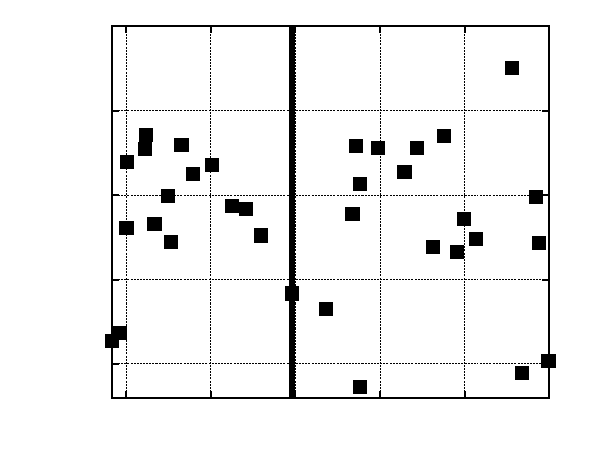
\includegraphics{CaelyxSucroseContinuousWAXSDiffraction}}%
    \gplfronttext
  \end{picture}%
\endgroup
}\label{fig:CaelyxSucroseContinuousWAXSDiffraction}}
		\caption{Measured in WAXS, the $q$-region where the doxorubicin diffraction peak appears can be observed. With black symbols, the shift of the doxorubicin-aggregate diffraction peak from $q=0.123$ nm$^{-1}$ is displayed The mean width (FWHM) is 0.333  nm$^{-1}$}
\end{figure}

To conclude this section, the diameter obtained from the isoscattering position in the aqueous iodixanol solution can be compared with what is measured in an aqueous sucrose suspending medium.  In the latter, if only the scattering curves below this osmolality threshold are considered, the relative standard deviation for each q value reveals a pronounced minimum for the first isoscattering point as depicted in Fig. 6. When comparing this result with the relative standard deviation curve obtained from the Optiprep TM contrast variation measurements, both values for the size of the drug carrier agree remarkably well within 0.8 $\%$. This reflects the independence of the technique from the contrast agent added to the suspending medium and shows the repeatability of the results.

\begin{figure}
	\centering
		\input{Figures/CaelyxIsopointComparison}
		\caption{Isoscattering point position quantified by the calculation of the relative standard deviation of the scattering curves for different solvent density gradients. In the case of the aqueous sucrose solution (black line), only the scattering curves below the osmolality threshold were employed for the calculation.}
		\label{fig:CaelyxIsopointComparison}
\end{figure}

\subsection{Size dependency of the osmotic activity}

\begin{figure}
	\centering
		\subfloat[Scattering curves]{\resizebox{0.44\linewidth}{!}{% GNUPLOT: LaTeX picture with Postscript
\begingroup
  \makeatletter
  \providecommand\color[2][]{%
    \GenericError{(gnuplot) \space\space\space\@spaces}{%
      Package color not loaded in conjunction with
      terminal option `colourtext'%
    }{See the gnuplot documentation for explanation.%
    }{Either use 'blacktext' in gnuplot or load the package
      color.sty in LaTeX.}%
    \renewcommand\color[2][]{}%
  }%
  \providecommand\includegraphics[2][]{%
    \GenericError{(gnuplot) \space\space\space\@spaces}{%
      Package graphicx or graphics not loaded%
    }{See the gnuplot documentation for explanation.%
    }{The gnuplot epslatex terminal needs graphicx.sty or graphics.sty.}%
    \renewcommand\includegraphics[2][]{}%
  }%
  \providecommand\rotatebox[2]{#2}%
  \@ifundefined{ifGPcolor}{%
    \newif\ifGPcolor
    \GPcolortrue
  }{}%
  \@ifundefined{ifGPblacktext}{%
    \newif\ifGPblacktext
    \GPblacktextfalse
  }{}%
  % define a \g@addto@macro without @ in the name:
  \let\gplgaddtomacro\g@addto@macro
  % define empty templates for all commands taking text:
  \gdef\gplbacktext{}%
  \gdef\gplfronttext{}%
  \makeatother
  \ifGPblacktext
    % no textcolor at all
    \def\colorrgb#1{}%
    \def\colorgray#1{}%
  \else
    % gray or color?
    \ifGPcolor
      \def\colorrgb#1{\color[rgb]{#1}}%
      \def\colorgray#1{\color[gray]{#1}}%
      \expandafter\def\csname LTw\endcsname{\color{white}}%
      \expandafter\def\csname LTb\endcsname{\color{black}}%
      \expandafter\def\csname LTa\endcsname{\color{black}}%
      \expandafter\def\csname LT0\endcsname{\color[rgb]{1,0,0}}%
      \expandafter\def\csname LT1\endcsname{\color[rgb]{0,1,0}}%
      \expandafter\def\csname LT2\endcsname{\color[rgb]{0,0,1}}%
      \expandafter\def\csname LT3\endcsname{\color[rgb]{1,0,1}}%
      \expandafter\def\csname LT4\endcsname{\color[rgb]{0,1,1}}%
      \expandafter\def\csname LT5\endcsname{\color[rgb]{1,1,0}}%
      \expandafter\def\csname LT6\endcsname{\color[rgb]{0,0,0}}%
      \expandafter\def\csname LT7\endcsname{\color[rgb]{1,0.3,0}}%
      \expandafter\def\csname LT8\endcsname{\color[rgb]{0.5,0.5,0.5}}%
    \else
      % gray
      \def\colorrgb#1{\color{black}}%
      \def\colorgray#1{\color[gray]{#1}}%
      \expandafter\def\csname LTw\endcsname{\color{white}}%
      \expandafter\def\csname LTb\endcsname{\color{black}}%
      \expandafter\def\csname LTa\endcsname{\color{black}}%
      \expandafter\def\csname LT0\endcsname{\color{black}}%
      \expandafter\def\csname LT1\endcsname{\color{black}}%
      \expandafter\def\csname LT2\endcsname{\color{black}}%
      \expandafter\def\csname LT3\endcsname{\color{black}}%
      \expandafter\def\csname LT4\endcsname{\color{black}}%
      \expandafter\def\csname LT5\endcsname{\color{black}}%
      \expandafter\def\csname LT6\endcsname{\color{black}}%
      \expandafter\def\csname LT7\endcsname{\color{black}}%
      \expandafter\def\csname LT8\endcsname{\color{black}}%
    \fi
  \fi
    \setlength{\unitlength}{0.0500bp}%
    \ifx\gptboxheight\undefined%
      \newlength{\gptboxheight}%
      \newlength{\gptboxwidth}%
      \newsavebox{\gptboxtext}%
    \fi%
    \setlength{\fboxrule}{0.5pt}%
    \setlength{\fboxsep}{1pt}%
\begin{picture}(5668.00,4534.00)%
    \gplgaddtomacro\gplbacktext{%
      \csname LTb\endcsname%
      \put(726,967){\makebox(0,0)[r]{\strut{}$1$}}%
      \csname LTb\endcsname%
      \put(726,1841){\makebox(0,0)[r]{\strut{}$10$}}%
      \csname LTb\endcsname%
      \put(726,2715){\makebox(0,0)[r]{\strut{}$100$}}%
      \csname LTb\endcsname%
      \put(726,3589){\makebox(0,0)[r]{\strut{}$1000$}}%
      \csname LTb\endcsname%
      \put(1359,484){\makebox(0,0){\strut{}$0.05$}}%
      \csname LTb\endcsname%
      \put(2040,484){\makebox(0,0){\strut{}$0.1$}}%
      \csname LTb\endcsname%
      \put(2720,484){\makebox(0,0){\strut{}$0.2$}}%
      \csname LTb\endcsname%
      \put(3620,484){\makebox(0,0){\strut{}$0.5$}}%
      \csname LTb\endcsname%
      \put(4300,484){\makebox(0,0){\strut{}$1$}}%
      \colorrgb{0.00,0.00,0.00}%
      \put(1256,1283){\makebox(0,0)[l]{\strut{}\fssmall \shortstack{Pseudo\\Isoscattering\\Point}}}%
    }%
    \gplgaddtomacro\gplfronttext{%
      \csname LTb\endcsname%
      \put(220,2266){\rotatebox{-270}{\makebox(0,0){\strut{}Scattering Intensity / a.u.}}}%
      \put(2639,154){\makebox(0,0){\strut{}$q$ / nm$^{-1}$}}%
      \csname LTb\endcsname%
      \put(4688,704){\makebox(0,0)[l]{\strut{}\fsmedium 0}}%
      \put(4688,1354){\makebox(0,0)[l]{\strut{}\fsmedium 5}}%
      \put(4688,2005){\makebox(0,0)[l]{\strut{}\fsmedium 10}}%
      \put(4688,2655){\makebox(0,0)[l]{\strut{}\fsmedium 15}}%
      \put(4688,3306){\makebox(0,0)[l]{\strut{}\fsmedium 20}}%
      \put(4688,3956){\makebox(0,0)[l]{\strut{}\fsmedium 25}}%
      \put(5018,2486){\rotatebox{-90}{\makebox(0,0){\strut{}\fsmedium Sucrose Mass Fraction / $\%$}}}%
    }%
    \gplbacktext
    \put(0,0){\includegraphics{SSLContinuousSAXS}}%
    \gplfronttext
  \end{picture}%
\endgroup
}\label{fig:SSLContinuousSAXS}}
		\subfloat[Isopoint intensity]{\resizebox{0.44\linewidth}{!}{\input{Figures/SSLIsopointIntensity}}\label{fig:SSLIsopointIntensity}}
		\caption{Scattering curves of SSL (50 nm, Oct 2015) measured at different solvent osmolalities with an aqueous sucrose density gradient. The osmotic shrinkage is quantified with the intensity of the isoscattering point at different osmolalities.}
\end{figure}






\begin{figure}
	\centering
		\subfloat[Scattering curves]{\resizebox{0.44\linewidth}{!}{\input{Figures/SSLCurveFeatureComparison}}\label{fig:SSLCurveFeatureComparison}}
		\subfloat[Bilayer deformation]{\resizebox{0.44\linewidth}{!}{\input{Figures/SSLBilayerDeformationChi2}}\label{fig:SSLBilayerDeformationChi2}}
		\caption{Scattering curve of SSL 50 nm (Oct 2015) in aqueous buffer and at maximum concentration. The phospholipid bilayer feature appears at $q>0.3$ nm$^{-1}$ and changes drastically from one curve to the other. At the right, the bilayer deformation is observed for increasing sucrose mass fraction e.g. solvent osmolality.}
\end{figure}


\begin{figure}
	\centering
		\subfloat[Poisson Law]{\resizebox{0.44\linewidth}{!}{\input{Figures/SSLPoissonOsmoticShrinkage}}\label{fig:SSLPoissonOsmoticShrinkage}}
		\subfloat[Bilayer deformation and osmotic shrinkage]{\resizebox{0.44\linewidth}{!}{% GNUPLOT: LaTeX picture with Postscript
\begingroup
  \makeatletter
  \providecommand\color[2][]{%
    \GenericError{(gnuplot) \space\space\space\@spaces}{%
      Package color not loaded in conjunction with
      terminal option `colourtext'%
    }{See the gnuplot documentation for explanation.%
    }{Either use 'blacktext' in gnuplot or load the package
      color.sty in LaTeX.}%
    \renewcommand\color[2][]{}%
  }%
  \providecommand\includegraphics[2][]{%
    \GenericError{(gnuplot) \space\space\space\@spaces}{%
      Package graphicx or graphics not loaded%
    }{See the gnuplot documentation for explanation.%
    }{The gnuplot epslatex terminal needs graphicx.sty or graphics.sty.}%
    \renewcommand\includegraphics[2][]{}%
  }%
  \providecommand\rotatebox[2]{#2}%
  \@ifundefined{ifGPcolor}{%
    \newif\ifGPcolor
    \GPcolortrue
  }{}%
  \@ifundefined{ifGPblacktext}{%
    \newif\ifGPblacktext
    \GPblacktextfalse
  }{}%
  % define a \g@addto@macro without @ in the name:
  \let\gplgaddtomacro\g@addto@macro
  % define empty templates for all commands taking text:
  \gdef\gplbacktext{}%
  \gdef\gplfronttext{}%
  \makeatother
  \ifGPblacktext
    % no textcolor at all
    \def\colorrgb#1{}%
    \def\colorgray#1{}%
  \else
    % gray or color?
    \ifGPcolor
      \def\colorrgb#1{\color[rgb]{#1}}%
      \def\colorgray#1{\color[gray]{#1}}%
      \expandafter\def\csname LTw\endcsname{\color{white}}%
      \expandafter\def\csname LTb\endcsname{\color{black}}%
      \expandafter\def\csname LTa\endcsname{\color{black}}%
      \expandafter\def\csname LT0\endcsname{\color[rgb]{1,0,0}}%
      \expandafter\def\csname LT1\endcsname{\color[rgb]{0,1,0}}%
      \expandafter\def\csname LT2\endcsname{\color[rgb]{0,0,1}}%
      \expandafter\def\csname LT3\endcsname{\color[rgb]{1,0,1}}%
      \expandafter\def\csname LT4\endcsname{\color[rgb]{0,1,1}}%
      \expandafter\def\csname LT5\endcsname{\color[rgb]{1,1,0}}%
      \expandafter\def\csname LT6\endcsname{\color[rgb]{0,0,0}}%
      \expandafter\def\csname LT7\endcsname{\color[rgb]{1,0.3,0}}%
      \expandafter\def\csname LT8\endcsname{\color[rgb]{0.5,0.5,0.5}}%
    \else
      % gray
      \def\colorrgb#1{\color{black}}%
      \def\colorgray#1{\color[gray]{#1}}%
      \expandafter\def\csname LTw\endcsname{\color{white}}%
      \expandafter\def\csname LTb\endcsname{\color{black}}%
      \expandafter\def\csname LTa\endcsname{\color{black}}%
      \expandafter\def\csname LT0\endcsname{\color{black}}%
      \expandafter\def\csname LT1\endcsname{\color{black}}%
      \expandafter\def\csname LT2\endcsname{\color{black}}%
      \expandafter\def\csname LT3\endcsname{\color{black}}%
      \expandafter\def\csname LT4\endcsname{\color{black}}%
      \expandafter\def\csname LT5\endcsname{\color{black}}%
      \expandafter\def\csname LT6\endcsname{\color{black}}%
      \expandafter\def\csname LT7\endcsname{\color{black}}%
      \expandafter\def\csname LT8\endcsname{\color{black}}%
    \fi
  \fi
  \setlength{\unitlength}{0.0500bp}%
  \begin{picture}(5668.00,4534.00)%
    \gplgaddtomacro\gplbacktext{%
      \csname LTb\endcsname%
      \put(1012,1014){\makebox(0,0)[r]{\strut{} 200}}%
      \csname LTb\endcsname%
      \put(1012,1402){\makebox(0,0)[r]{\strut{} 250}}%
      \csname LTb\endcsname%
      \put(1012,1789){\makebox(0,0)[r]{\strut{} 300}}%
      \csname LTb\endcsname%
      \put(1012,2177){\makebox(0,0)[r]{\strut{} 350}}%
      \csname LTb\endcsname%
      \put(1012,2564){\makebox(0,0)[r]{\strut{} 400}}%
      \csname LTb\endcsname%
      \put(1012,2952){\makebox(0,0)[r]{\strut{} 450}}%
      \csname LTb\endcsname%
      \put(1012,3339){\makebox(0,0)[r]{\strut{} 500}}%
      \csname LTb\endcsname%
      \put(1012,3727){\makebox(0,0)[r]{\strut{} 550}}%
      \csname LTb\endcsname%
      \put(1012,4114){\makebox(0,0)[r]{\strut{} 600}}%
      \csname LTb\endcsname%
      \put(1144,484){\makebox(0,0){\strut{} 0.014}}%
      \csname LTb\endcsname%
      \put(1894,484){\makebox(0,0){\strut{} 0.016}}%
      \csname LTb\endcsname%
      \put(2645,484){\makebox(0,0){\strut{} 0.018}}%
      \csname LTb\endcsname%
      \put(3395,484){\makebox(0,0){\strut{} 0.02}}%
      \csname LTb\endcsname%
      \put(4145,484){\makebox(0,0){\strut{} 0.022}}%
      \csname LTb\endcsname%
      \put(4896,484){\makebox(0,0){\strut{} 0.024}}%
      \put(176,2486){\rotatebox{-270}{\makebox(0,0){\strut{}Pressure difference / mOsm kg$^{-1}$}}}%
      \put(3339,154){\makebox(0,0){\strut{}1/Radius / nm$^{-1}$}}%
      \colorrgb{0.00,0.00,0.00}%
      \put(2270,1324){\makebox(0,0)[l]{\strut{}Osmotic Shrinkage}}%
      \colorrgb{0.80,0.31,0.31}%
      \put(3770,3107){\makebox(0,0)[l]{\strut{}HSPC+PEG}}%
      \colorrgb{0.43,0.42,0.82}%
      \put(1894,3727){\makebox(0,0)[l]{\strut{}HSPC}}%
      \colorrgb{0.00,0.00,0.00}%
      \put(3770,2254){\makebox(0,0)[l]{\strut{}Caelyx}}%
    }%
    \gplgaddtomacro\gplfronttext{%
    }%
    \gplbacktext
    \put(0,0){\includegraphics{SSLPoissonComplete}}%
    \gplfronttext
  \end{picture}%
\endgroup
}\label{fig:SSLPoissonComplete}}
		\caption{Summary of the different osmotic pressures needed for the deformation of the liposamal structure. The radius was determined by DLS.}
\end{figure}







\section{Application to blood plasma componenents}
\subsection{HDL}
\subsection{LDL}
\subsection{Literature comparison}

\section{Protein-coated low-density nanoparticles}
\subsection{Singe-contrast SAXS}
Caterina Minelli Paper ECASIA
\subsection{Contrast variation}
Isopoint subtraction, as in BioSurf

\section{Summary}
This article demonstrates that it is possible to determine the size of a PEGylated liposomal drug carrier with continuous contrast variation in SAXS. By means of an iso-osmolal density gradient, the position of the isoscattering point was measured whereby the size of the liposomal drug was determined. Supplemented by the model fitting of the so called shape factor of the liposomes, the size was also obtained from an independent evaluation procedure and an average size of (69 $\pm$ 5) nm was obtained. This size is smaller than the value measured by DLS, which can be attributed to the fact that the contrast variation SAXS determines the size of the liposomes impermeable to the contrast agent, i.e. the outer PEG layer of the liposomes is not probed. The latter implies that the combination of SAXS with DLS can reveal the difference between the hydrodynamic diameter and the "core" size of the nanocarrier, which is related to the thickness of the PEG-layer in case of stealth liposomes. Moreover the method presented in this paper shows that by means of the shape factor fitting, complementary information about the shape of the nanocarrier can be obtained.

Using an aqueous sucrose density gradient, it was shown that an increasing osmolality of the buffer produces an osmotic shrinkage of the liposomal structure, although this structural deformation is reversible and does not affect the crystalline structure of the intraliposomal doxorubicin.

These results, together with the determination of the average electron density of the liposomal doxorubicin of (346.2 $\pm$ 1.2) nm$^{-3}$, demonstrate the applicability of the density gradient technique for complex particles. This model-free approach to contrast variation in SAXS proves to be a powerful sizing technique, which, in addition, makes it possible to study simultaneously the behavior of the liposomal drug carrier under different osmotic conditions.


	
		
	\bibliography{thesis}%,main}%,iucr, polymers,polymers_patent,iucr}
	
	%       main.bib contains possible references for new parts of the thesis
	
	\pagestyle{empty}
\noindent
\section*{Acknowledgments}

\textcolor{red}{STILL TO WRITE!!!!}
\vspace{2ex}

The conclusion of this Master Thesis would have been impossible without the help of so many people, who I would like in this opportunity to thank and acknowledge here.
\vspace{2ex}

\noindent Laborortory of the Physikalisch-Technischen Bundesanstalt (PTB) in Electron Storage Ring BESSY II from Helmholtz-Zentrum Berlin (HZB),
\vspace{2ex}

\noindent First of all, I would like to thank my supervisor Dr. Michael Krumrey, the person who made possible this Thesis happening. It has been a great opportunity for me to be part of this team, Rontgen Metrologie, which provided me the chance to make high-profile experiments and a proper environment to develop my goals. Without the supervision, expert adivse and suggestions of Dr. Krumrey, the satisfactory achievement of this thesis’s goals would have been impossible.
\vspace{2ex}

\noindent Prof. Dr. Mathias Richter,
\vspace{2ex}

\noindent Prof. Dr. Stefan Eisebitt und Prof. Dr. Simone Raoux,
\vspace{2ex}

\noindent I would like also to thank Dr. Christian Gollwitzer for his supervision and honest interest during this time together, giving me very valuable scientific input.
\vspace{2ex}

\noindent Arbeitsgruppe 7.11 Levent Cibik, Ulf Knoll, Stefanie Langner, Swenja Schreiber, Layla Riemann und Peter Müller,
\vspace{2ex}

\noindent Dr. Jan Wernecke, Analia Fernandez-Herrero, Anton Haase, Mika Pflüger and Dr. Viktor Soltwisch, make a good day out of a bad one. 
\vspace{2ex}

\noindent Dr. Zoltan Varga from the Institute of Materials and Environmental Chemistry, Research Centre for Natural Sciences (MTA),
\vspace{2ex}

\noindent Dr. Caterina Minelli, Dr. Aneta Sikora and Dr. Alex Shard from National Physical Laboratory (NPL),
\vspace{2ex}

\noindent Dr. Armin Hoell from HZB,
\vspace{2ex}

\noindent Eike Gericke and Roland Schmack for the SBA measurements,
\vspace{2ex}

\noindent My HZB colleagues for interesting scientific comments Dr. Kaan Atak, Dr. Wilson Quevedo,
\vspace{2ex}

\noindent My physics and non-physics friends Dr. Markus Krecik, Alexander Humeniuk, Alessandro Riccotone, Alisio Delgado, Alberto Gurkensaft and the Margon's 12,
\vspace{2ex}

\noindent And of course, a warm and honest thanks to my Family, to my Parents and to Marta, who haven't let me down at any point, neither physically nor mentally. Gracias por estar siempre ahí, donde y cuando se os necesita.

\cleardoublepage

	
	\selectlanguage{ngerman}

\section*{Eidesstattliche Versicherung}
\vspace{3ex}

Hiermit versichere ich an Eides statt, dass ich die vorliegende Arbeit selbstständig verfasst und keine anderen als die in der Dissertation angegebenen Quellen und Hilfsmittel benutzt habe.
Alle Ausführungen, die anderen veröffentlichten oder nicht veröffentlichten Schriften wörtlich oder sinngemäß entnommen wurden, habe ich kenntlich gemacht.
Die Darstellung des Eigenanteils an bereits publizierten Inhalten in meiner beigefügten Erklärung ist zutreffend.

Es gab keine Zusammenarbeit mit anderen wissenschaftlichen Mitarbeitern, die ein Promotionsverfahren anstreben.

\vspace{3cm}

\noindent Berlin, den 15. Februar 2017 \hfill Raül Garc\'{i}a Diez

\cleardoublepage


	
\end{document}
